%=============================================================================
% Thesis Template in LaTex
%
% File:  Anhang.tex -- Anhang
% Author(s): Cyrano Golliez <golliezc@student.ethz.ch>
%
% Creation:  27 Jan 2014
% Time-stamp: <Tue 2013-08-13 20:14 juergen>
%
% Copyright (c) 2014 Infrastructure Management Group (IMG)
%               http://ibi.ethz.ch
%
% More information on LaTeX: http://www.latex-project.org/
%=============================================================================

%----Kostenberechnung der Varianten---------

\begin{figure}[h!]
	\centering
	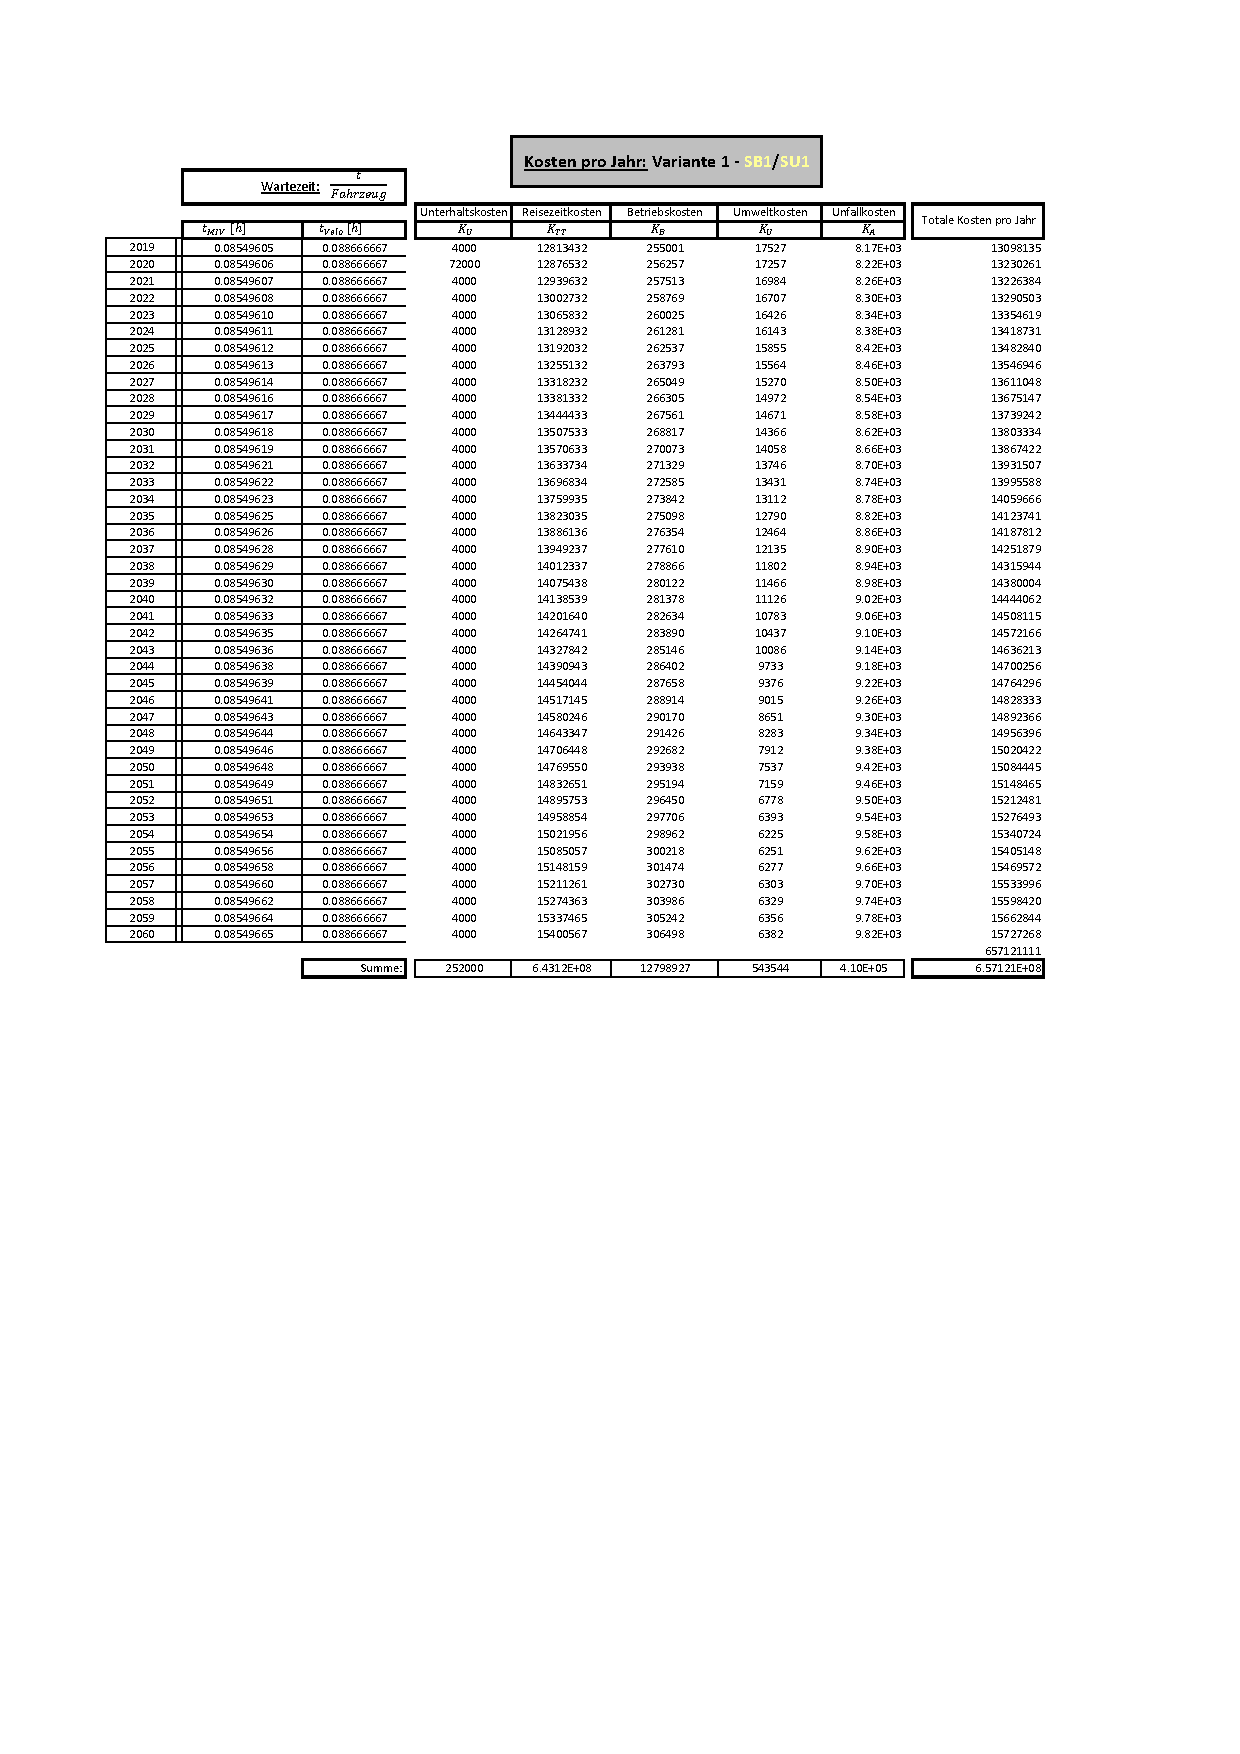
\includegraphics[width=\textwidth]{figures/Anhang/f-00-A-V1-B1-U1}
	\caption{Kostenberechung Variante 1 - SB1/SU1}
\end{figure}

\begin{figure}[h!]
	\centering
	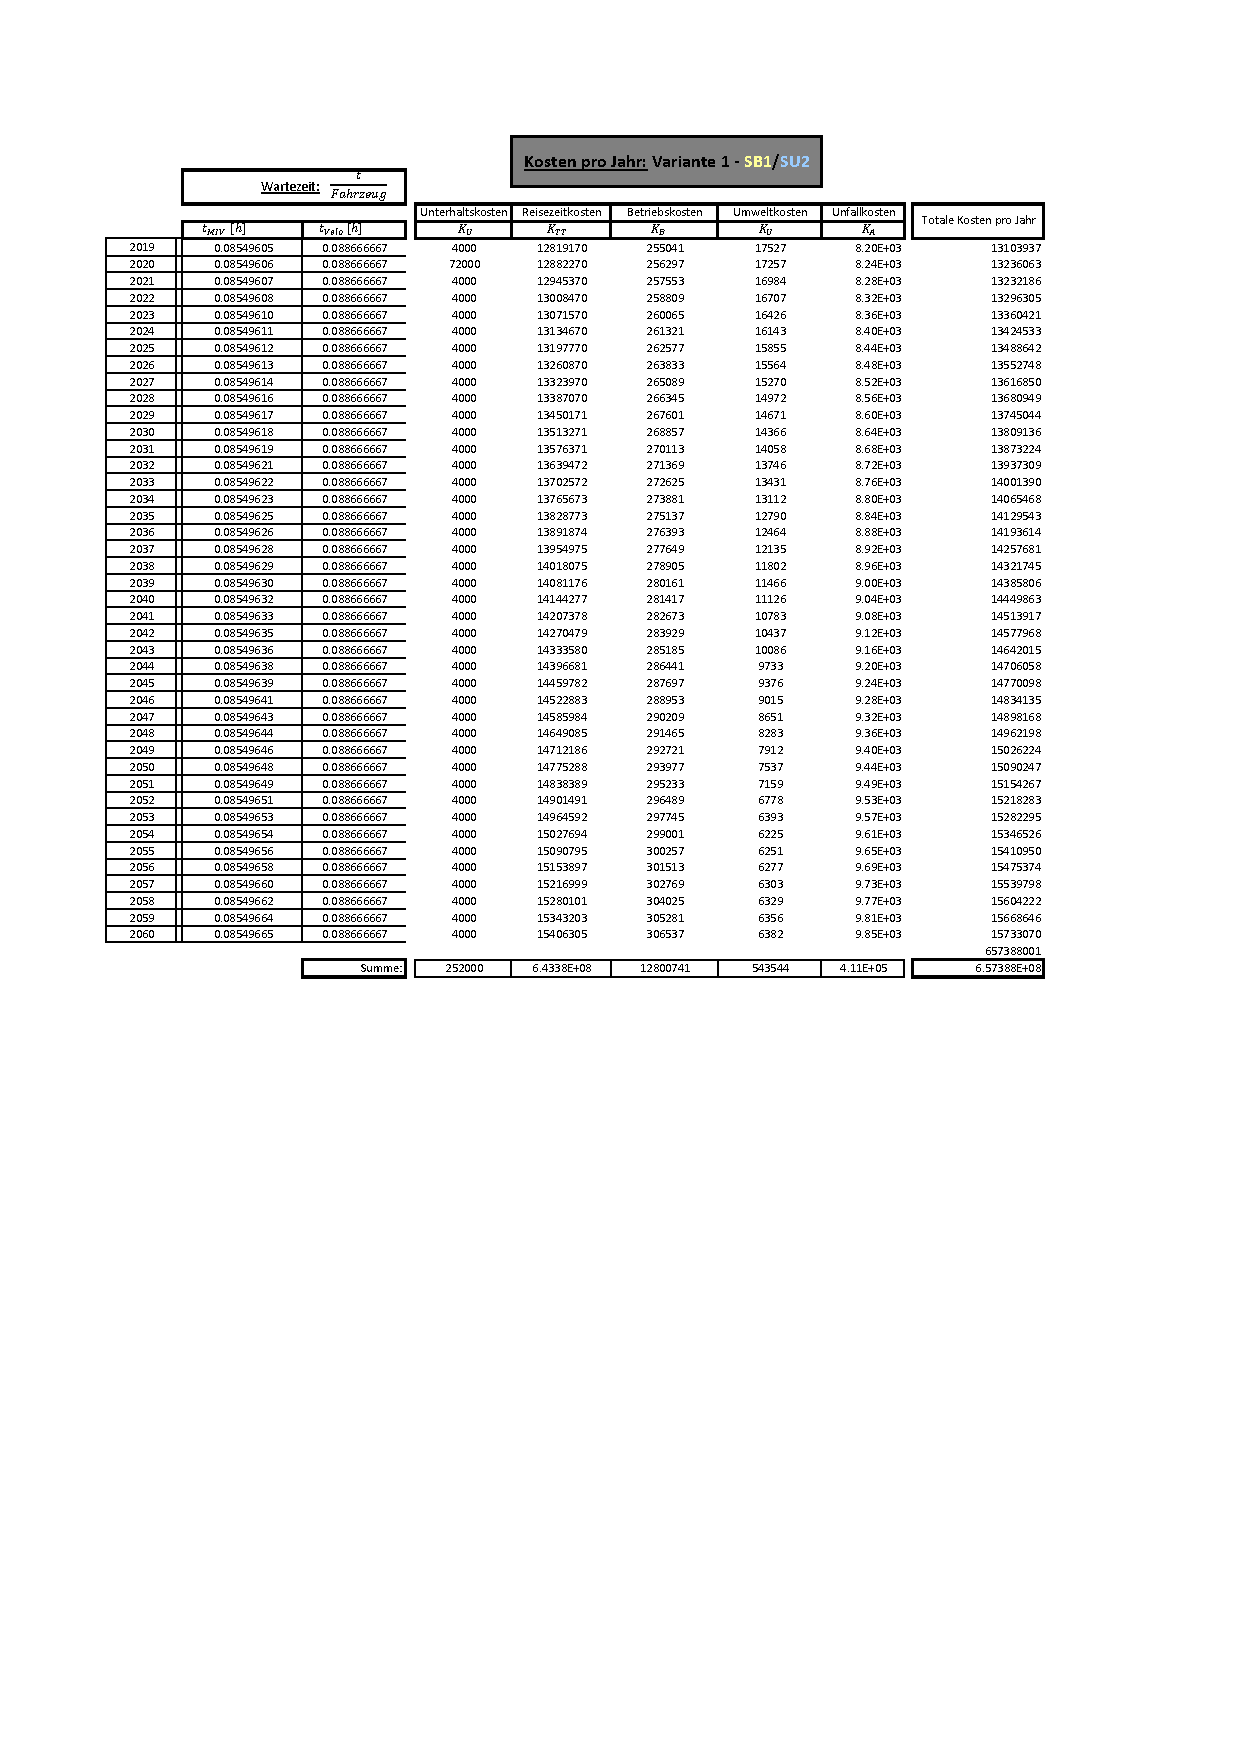
\includegraphics[width=\textwidth]{figures/Anhang/f-00-A-V1-B1-U2}
	\caption{Kostenberechung Variante 1 - SB1/SU2}
\end{figure}

\begin{figure}[h!]
	\centering
	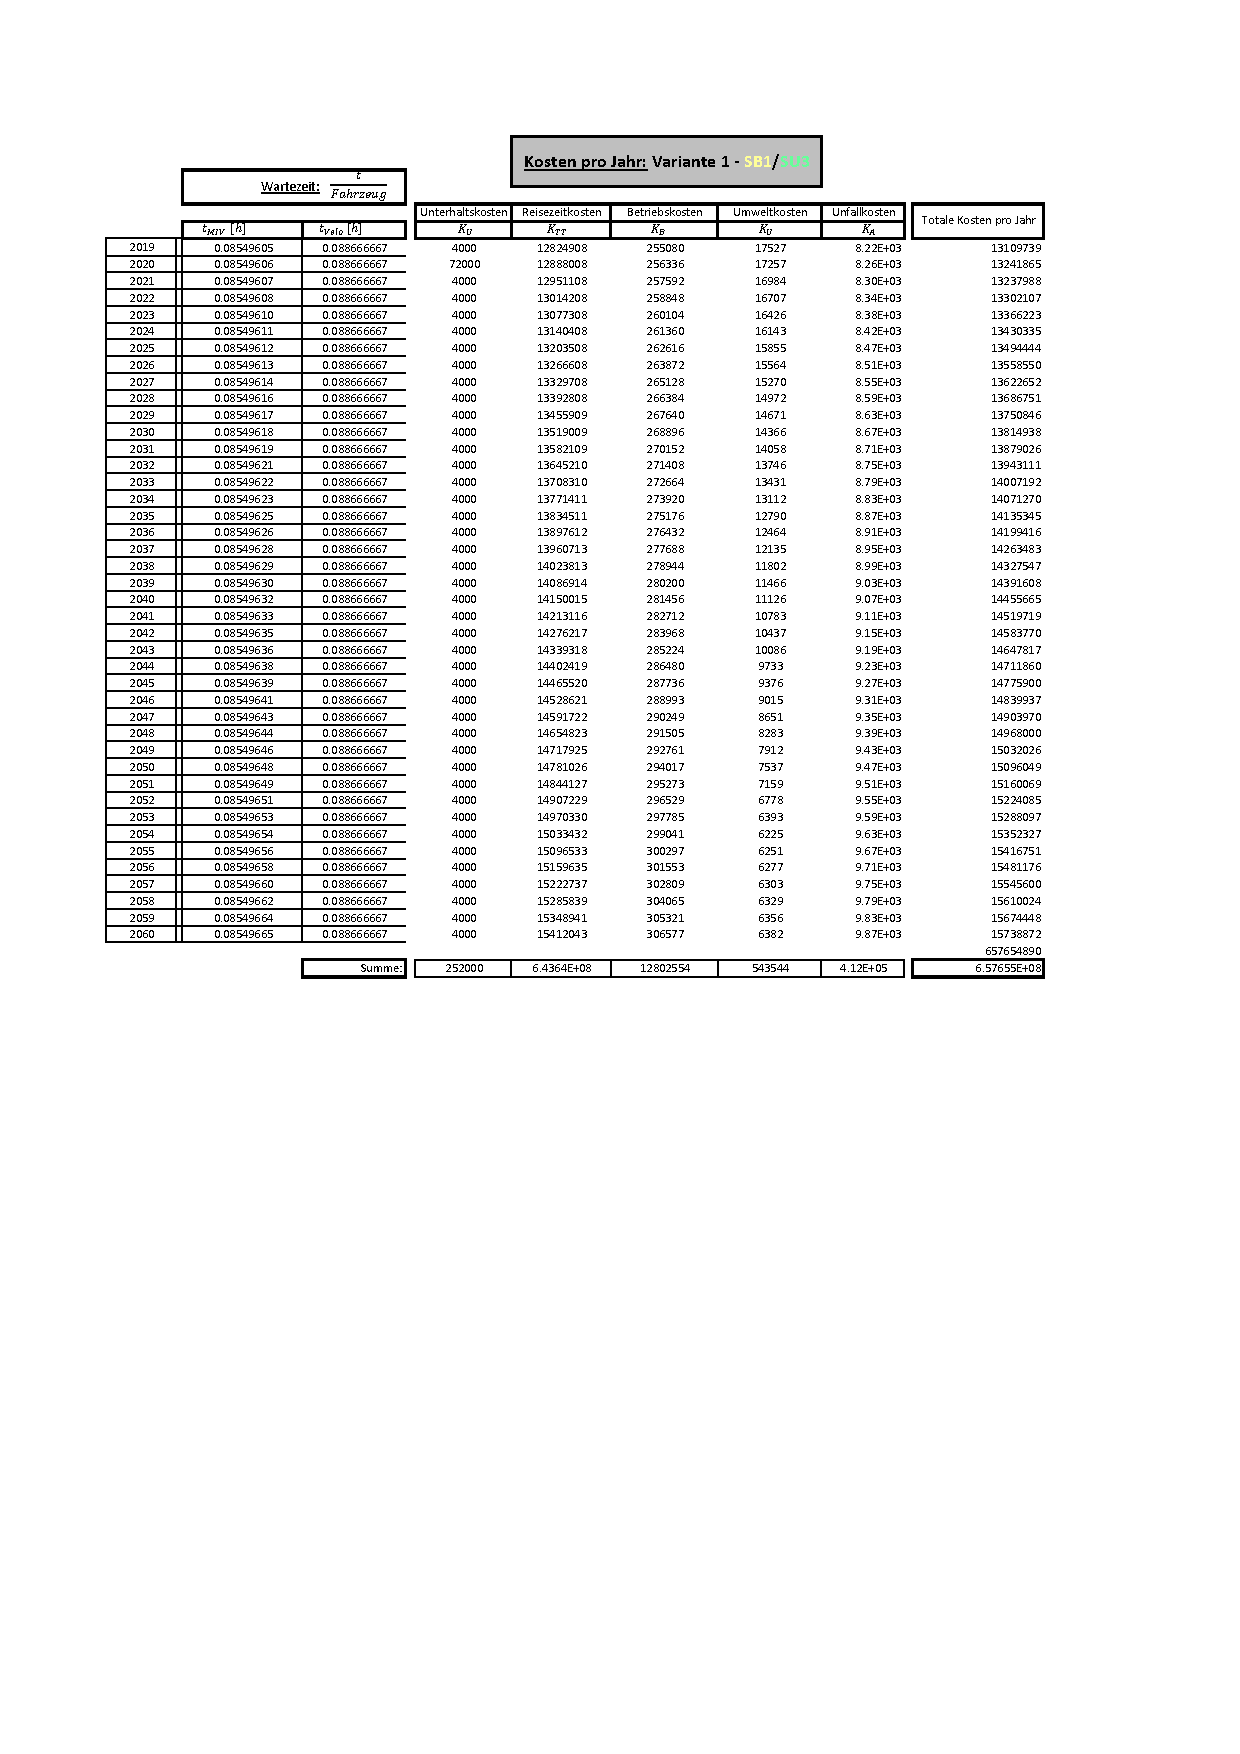
\includegraphics[width=\textwidth]{figures/Anhang/f-00-A-V1-B1-U3}
	\caption{Kostenberechung Variante 1 - SB1/SU3}
\end{figure}

\begin{figure}[h!]
	\centering
	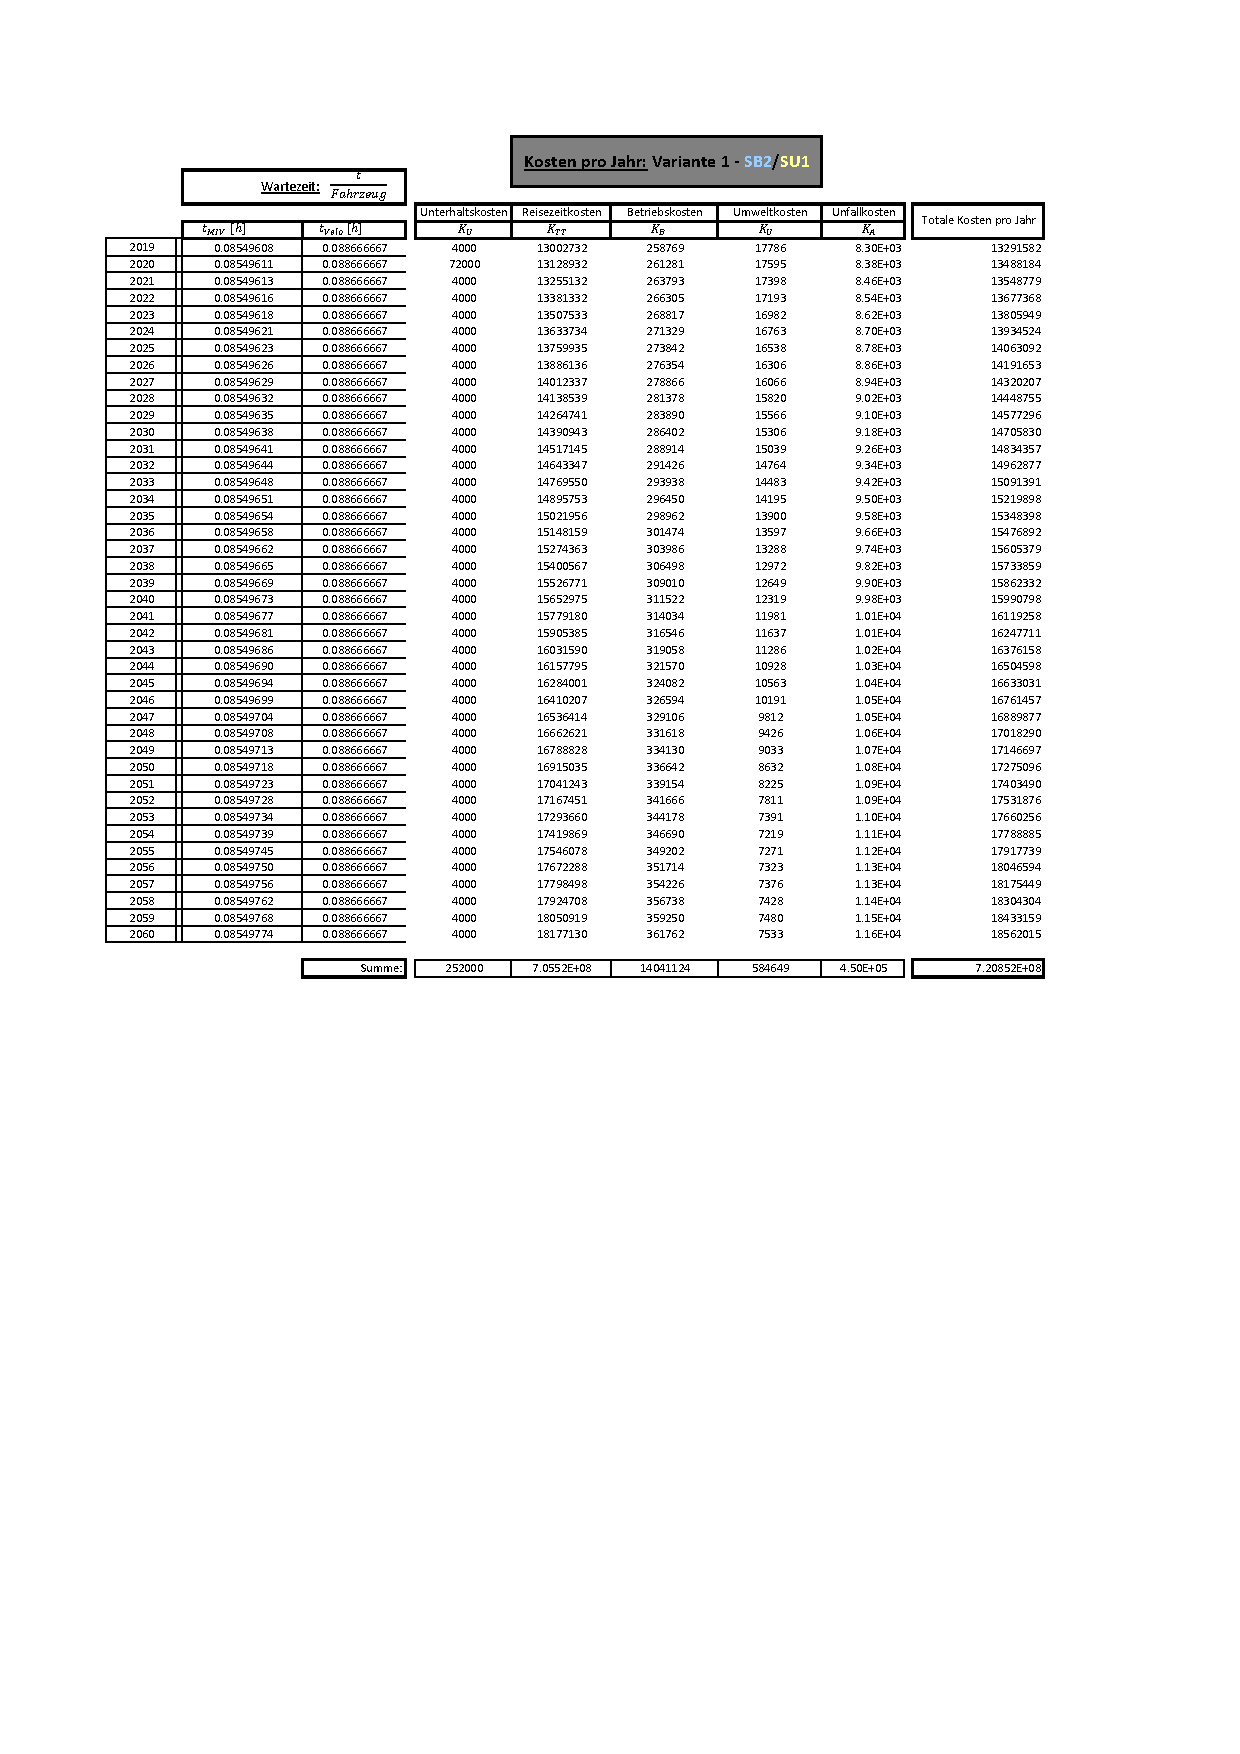
\includegraphics[width=\textwidth]{figures/Anhang/f-00-A-V1-B2-U1}
	\caption{Kostenberechung Variante 1 - SB2/SU1}
\end{figure}

\begin{figure}[h!]
	\centering
	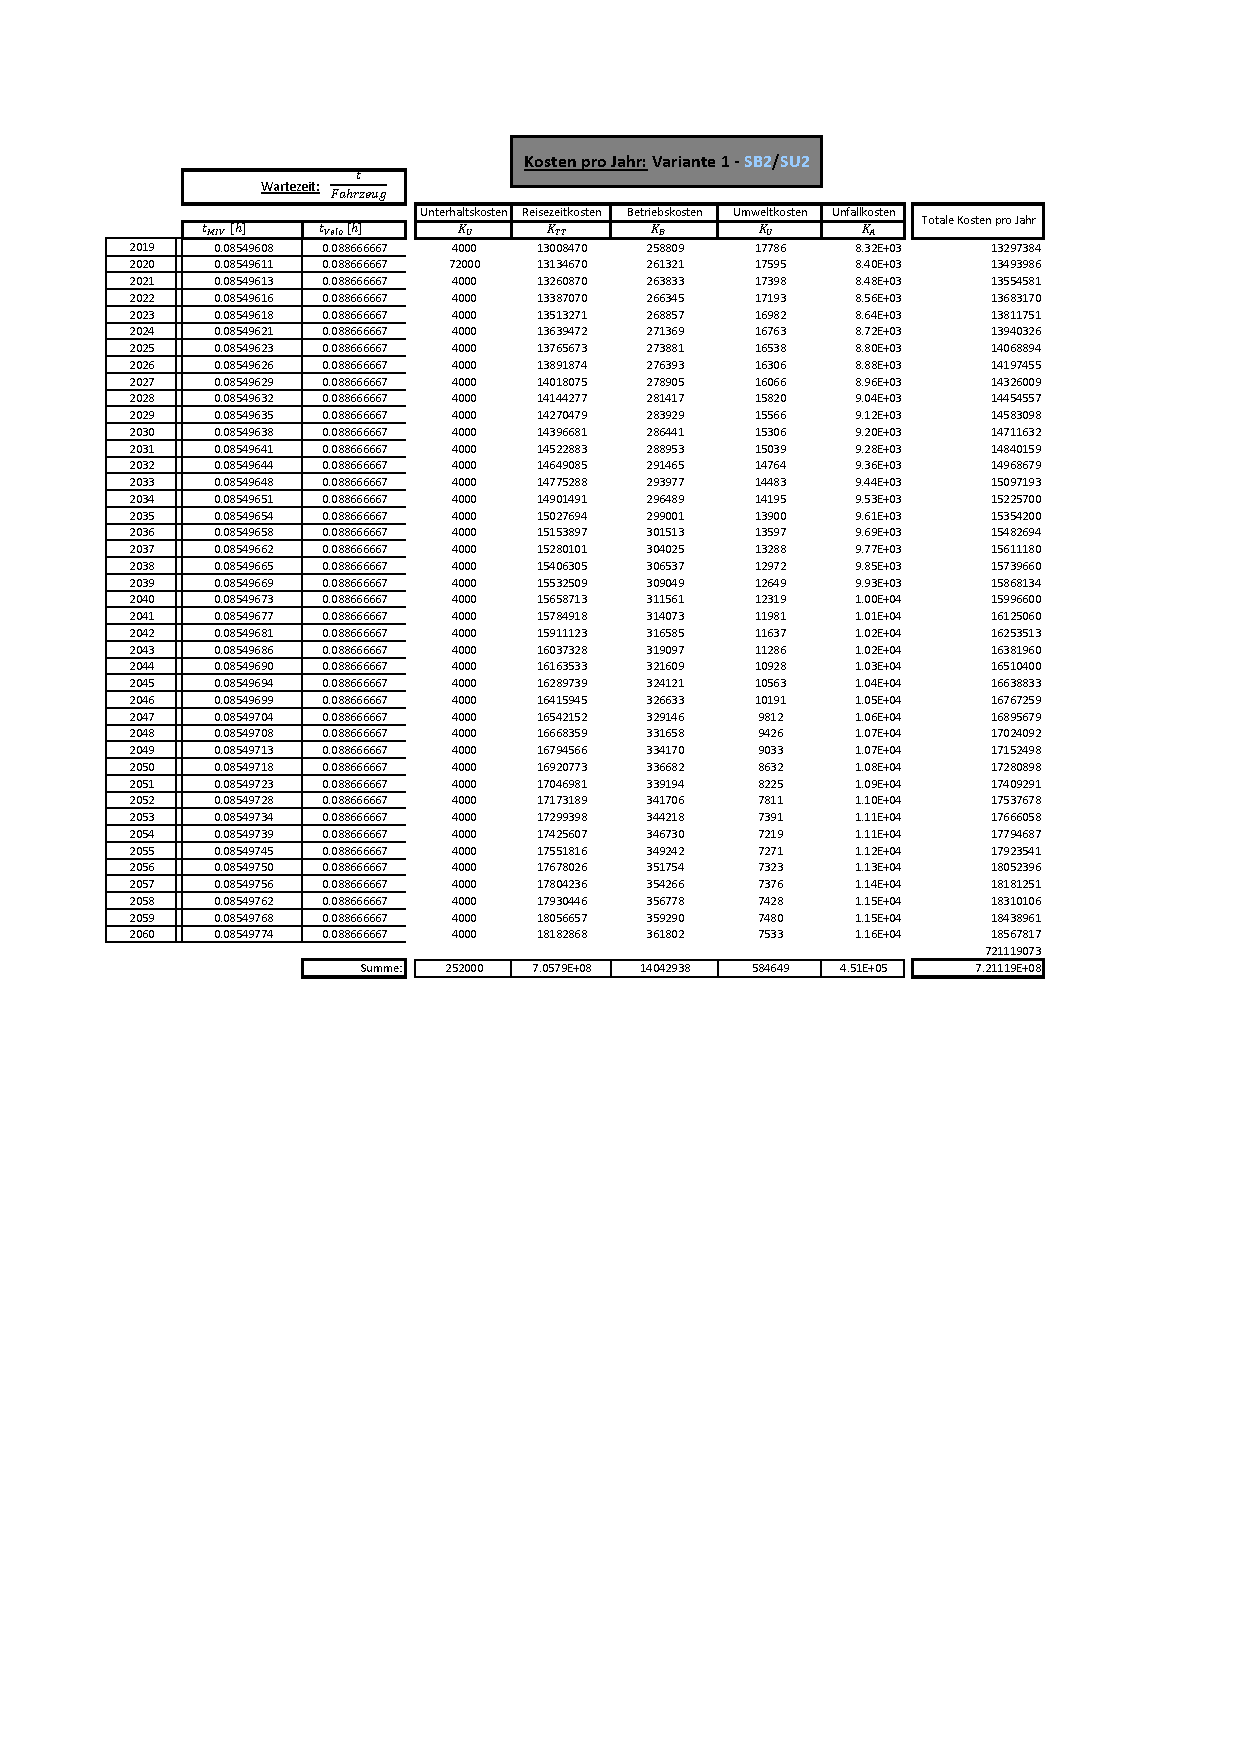
\includegraphics[width=\textwidth]{figures/Anhang/f-00-A-V1-B2-U2}
	\caption{Kostenberechung Variante 1 - SB2/SU2}
\end{figure}

\begin{figure}[h!]
	\centering
	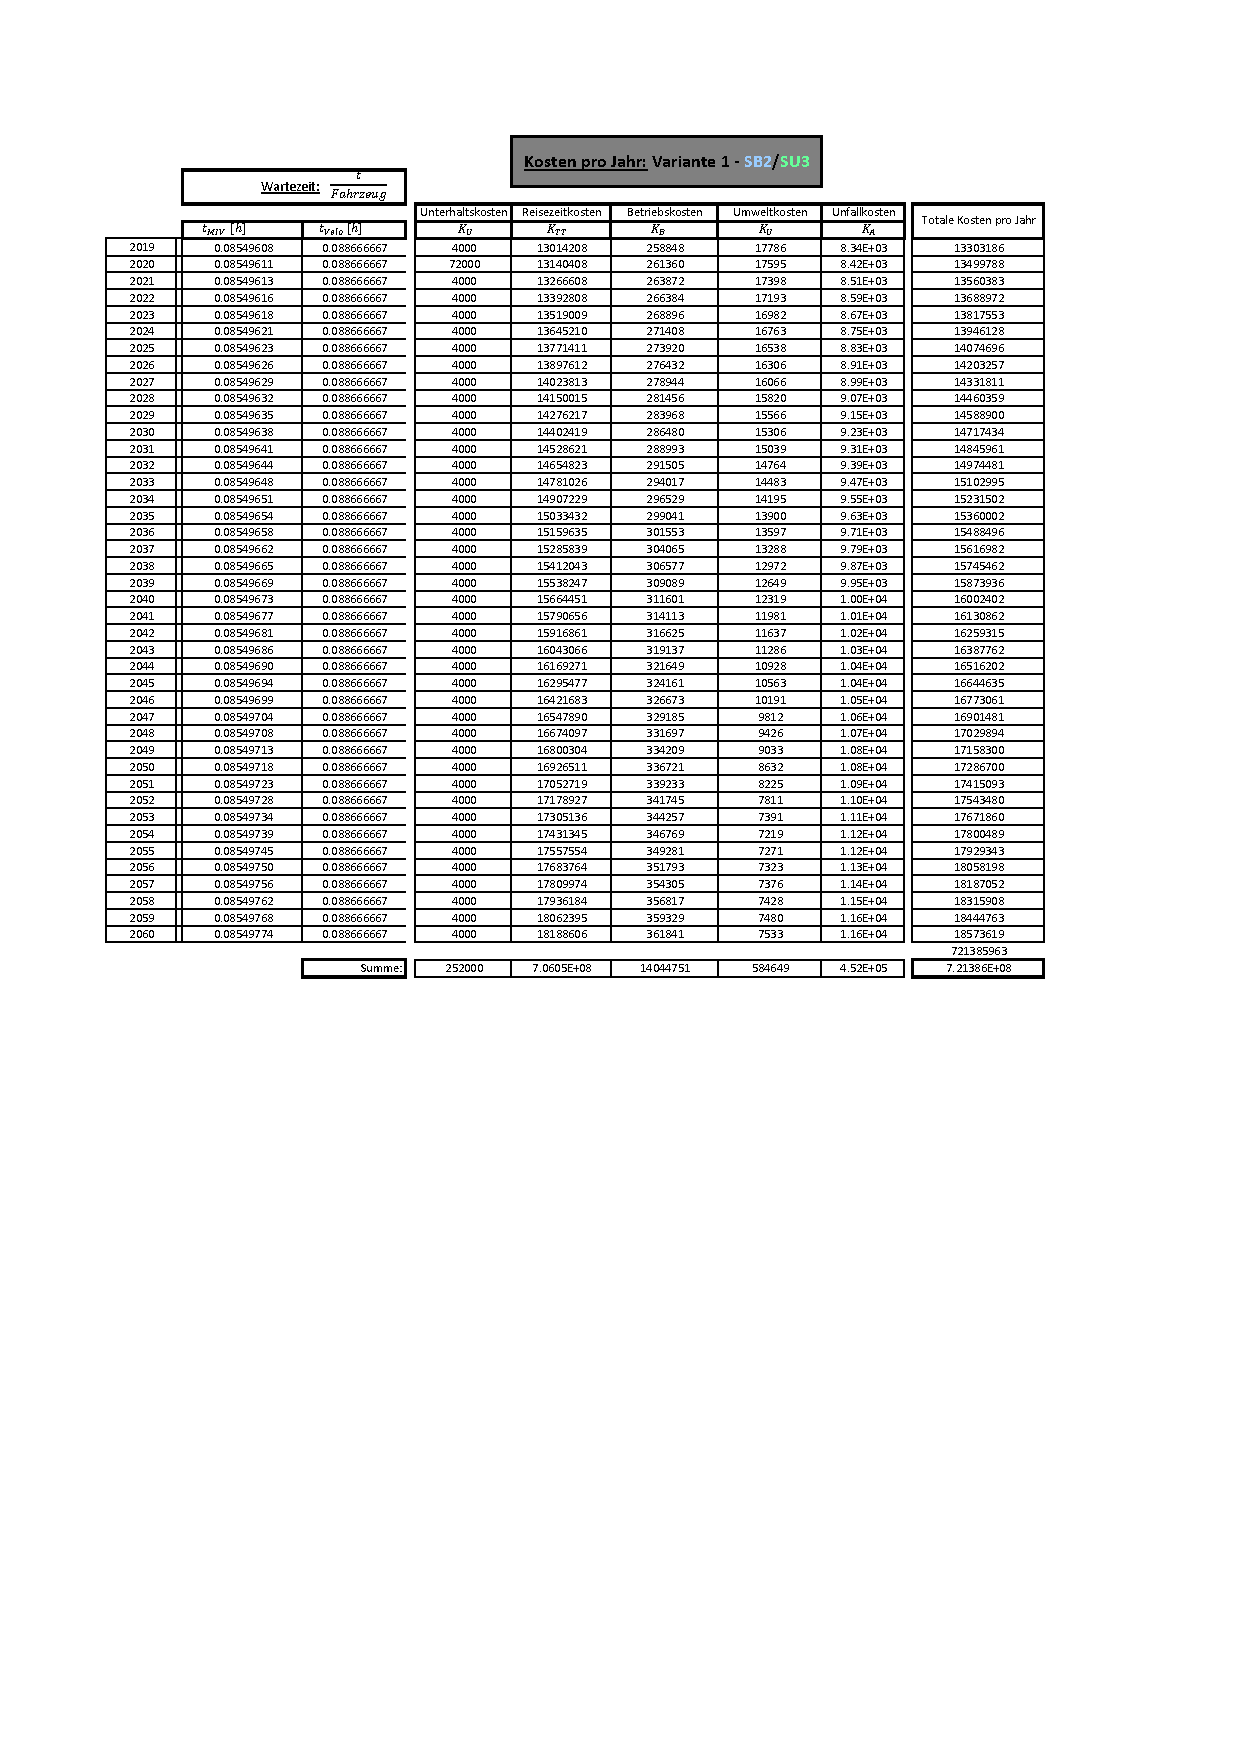
\includegraphics[width=\textwidth]{figures/Anhang/f-00-A-V1-B2-U3}
	\caption{Kostenberechung Variante 1 - SB2/SU3}
\end{figure}

\begin{figure}[h!]
	\centering
	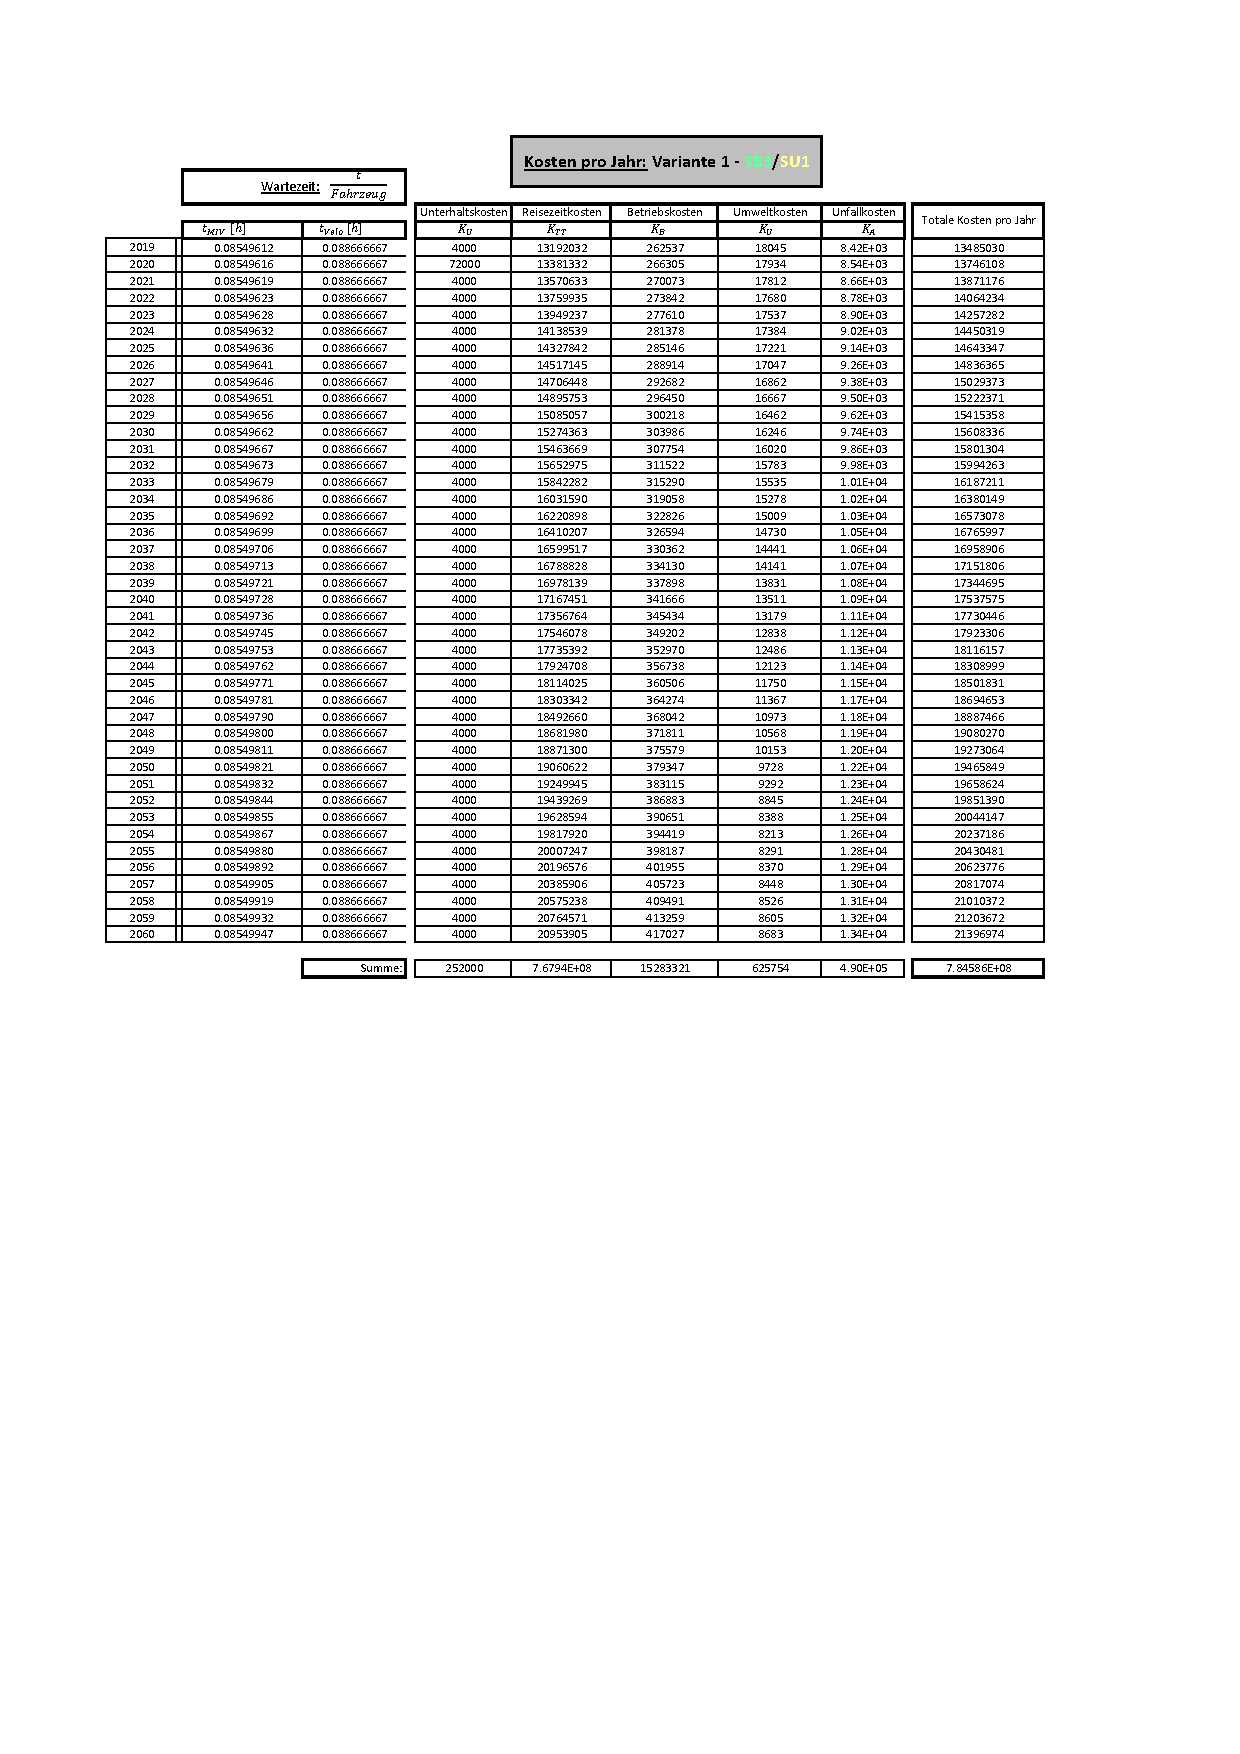
\includegraphics[width=\textwidth]{figures/Anhang/f-00-A-V1-B3-U1}
	\caption{Kostenberechung Variante 1 - SB3/SU1}
\end{figure}

\begin{figure}[h!]
	\centering
	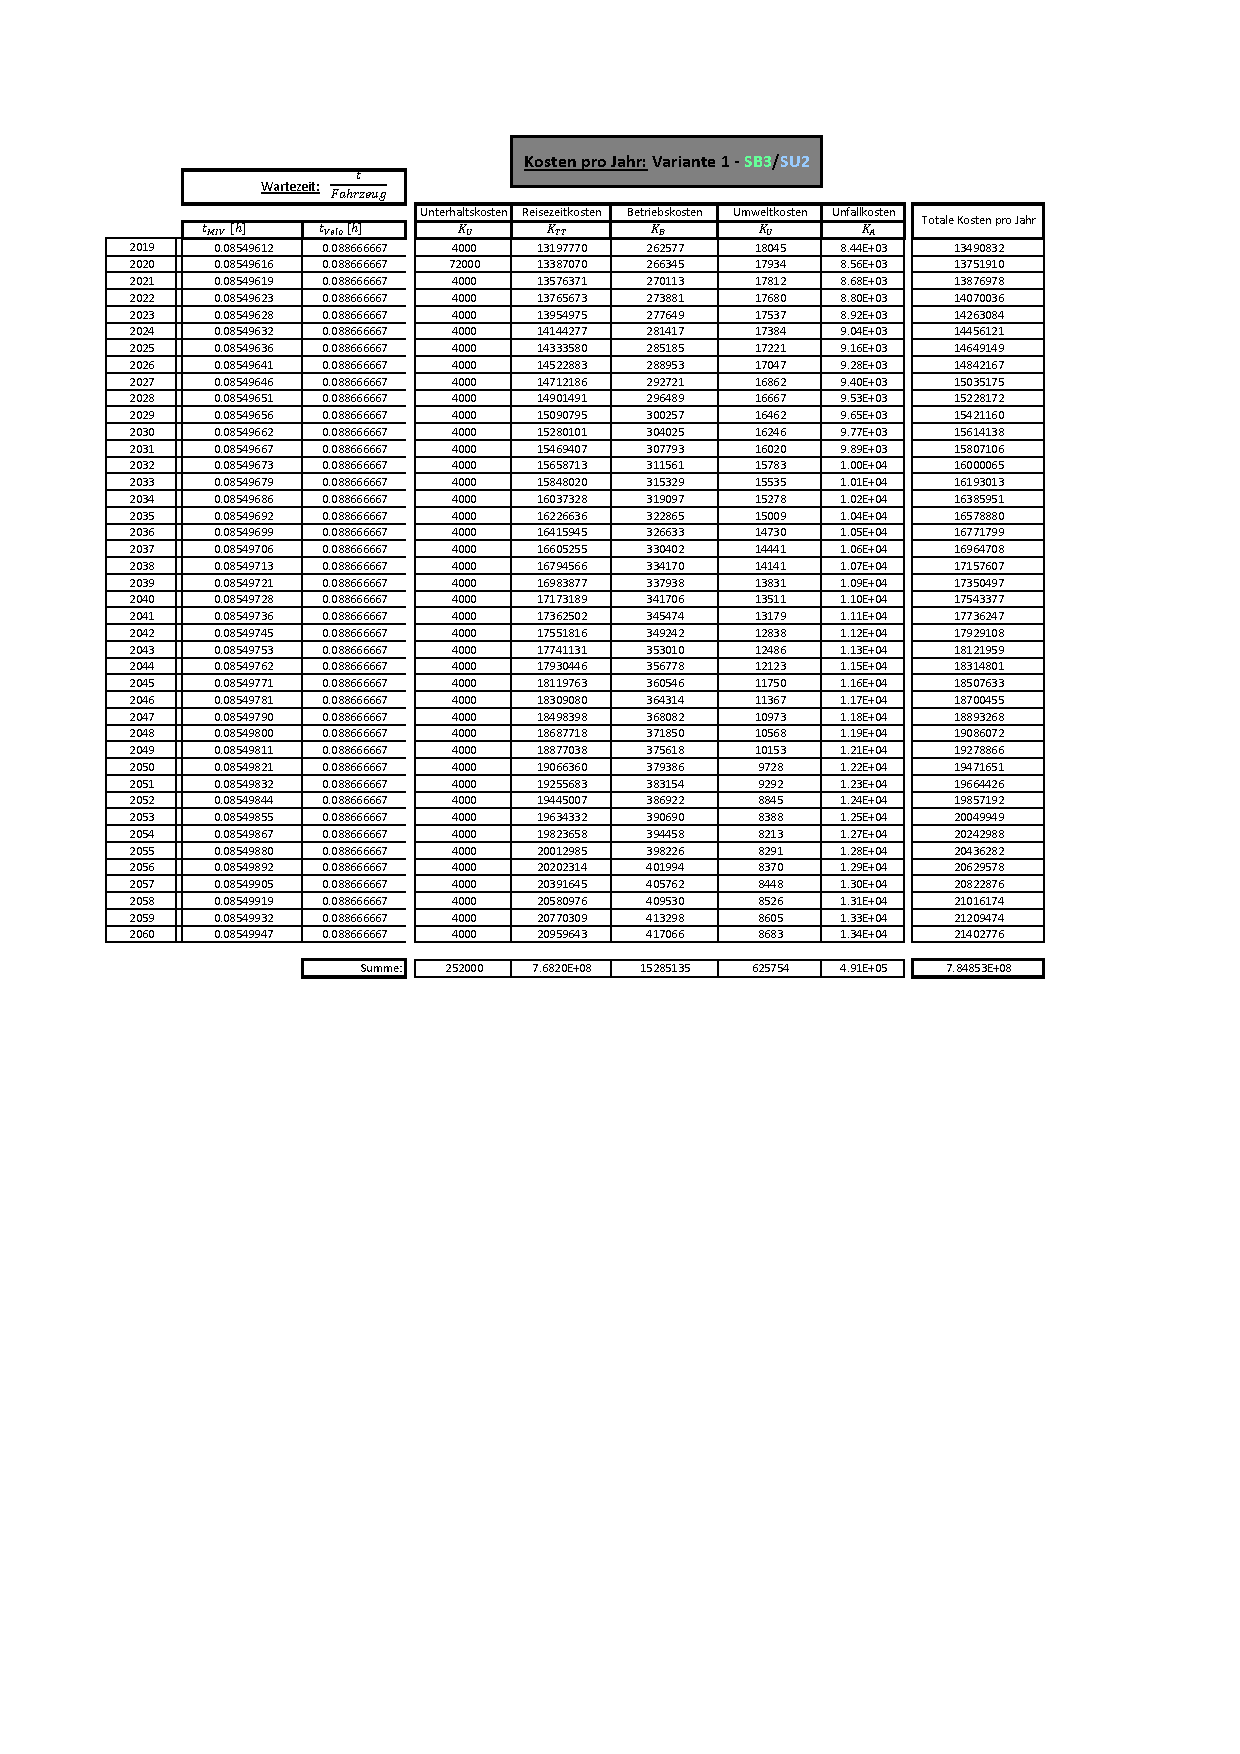
\includegraphics[width=\textwidth]{figures/Anhang/f-00-A-V1-B3-U2}
	\caption{Kostenberechung Variante 1 - SB3/SU2}
\end{figure}

\begin{figure}[h!]
	\centering
	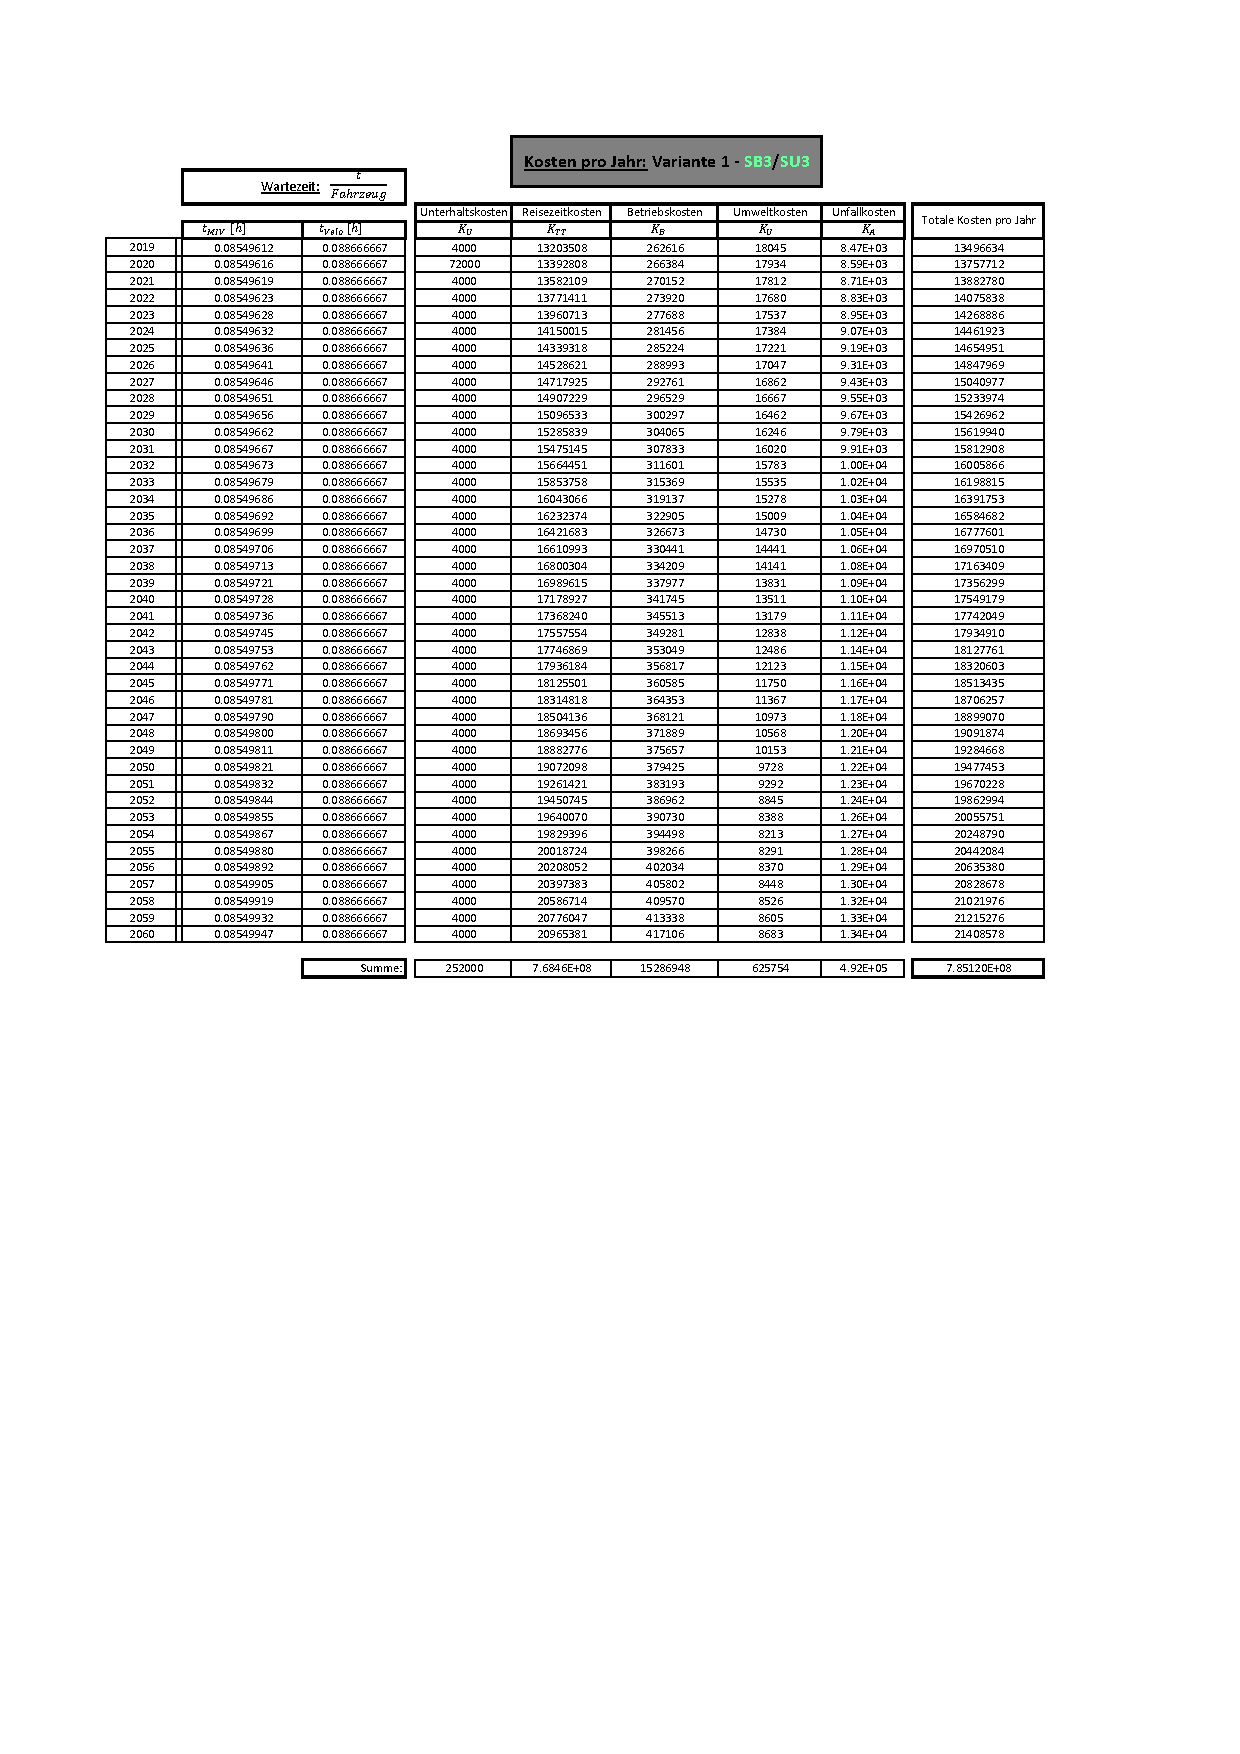
\includegraphics[width=\textwidth]{figures/Anhang/f-00-A-V1-B3-U3}
	\caption{Kostenberechung Variante 1 - SB3/SU3}
\end{figure}

\begin{figure}[h!]
	\centering
	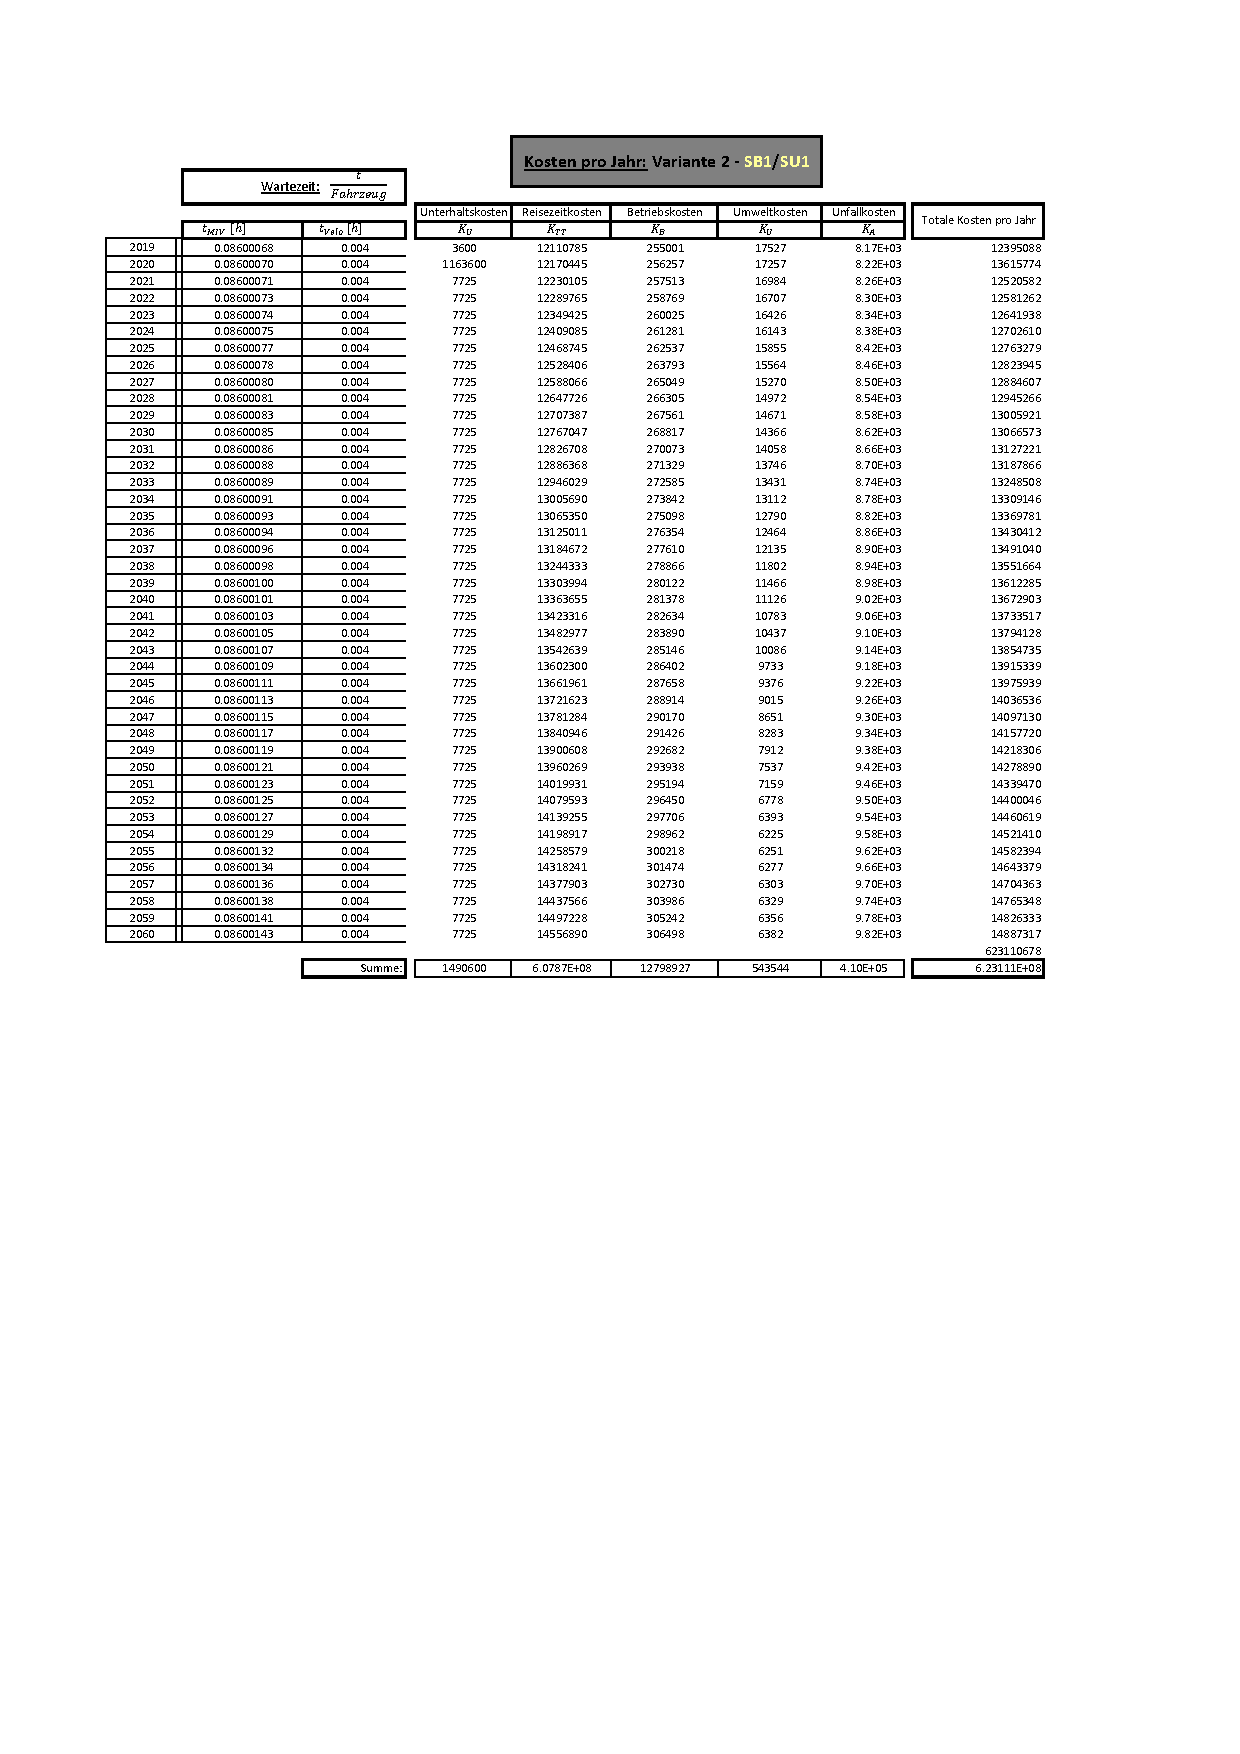
\includegraphics[width=\textwidth]{figures/Anhang/f-00-A-V2-B1-U1}
	\caption{Kostenberechung Variante 2 - SB1/SU1}
\end{figure}

\begin{figure}[h!]
	\centering
	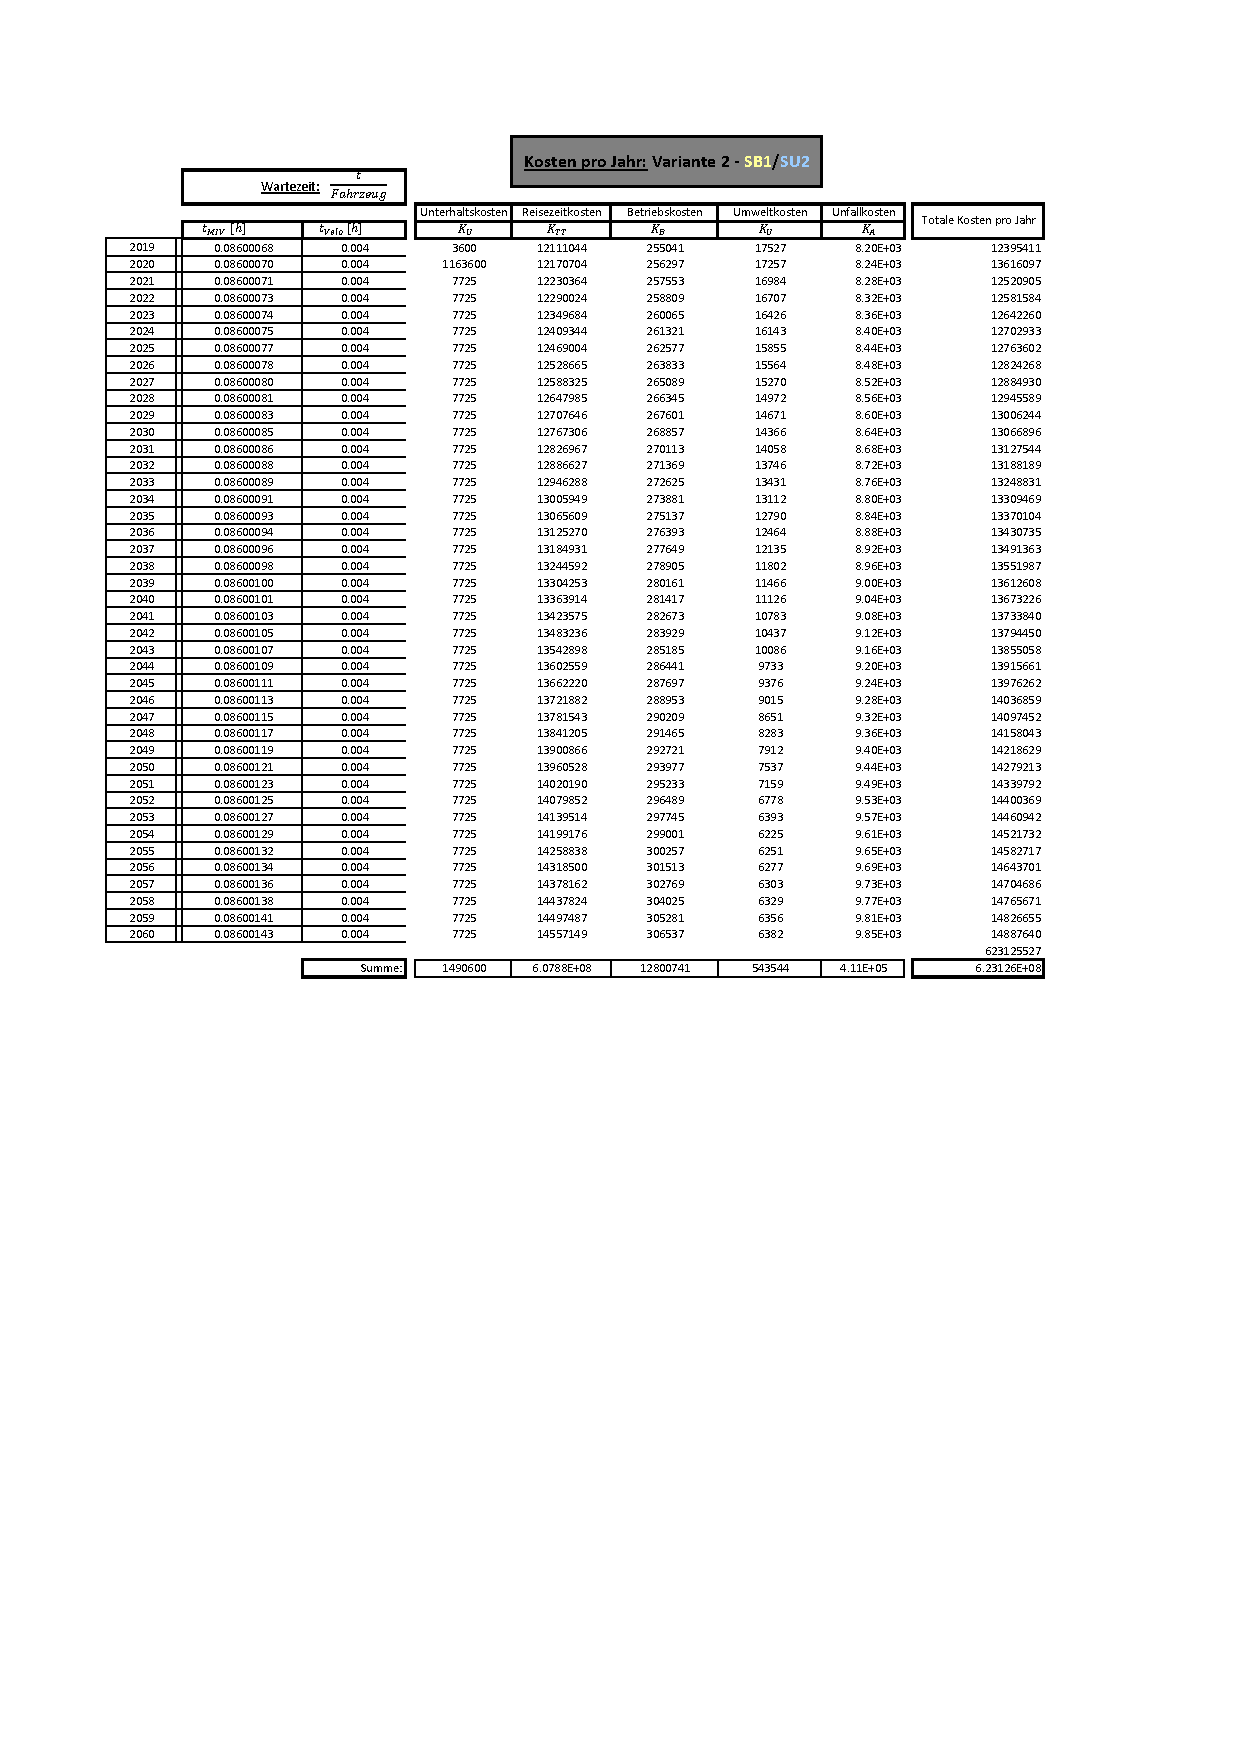
\includegraphics[width=\textwidth]{figures/Anhang/f-00-A-V2-B1-U2}
	\caption{Kostenberechung Variante 2 - SB1/SU2}
\end{figure}

\begin{figure}[h!]
	\centering
	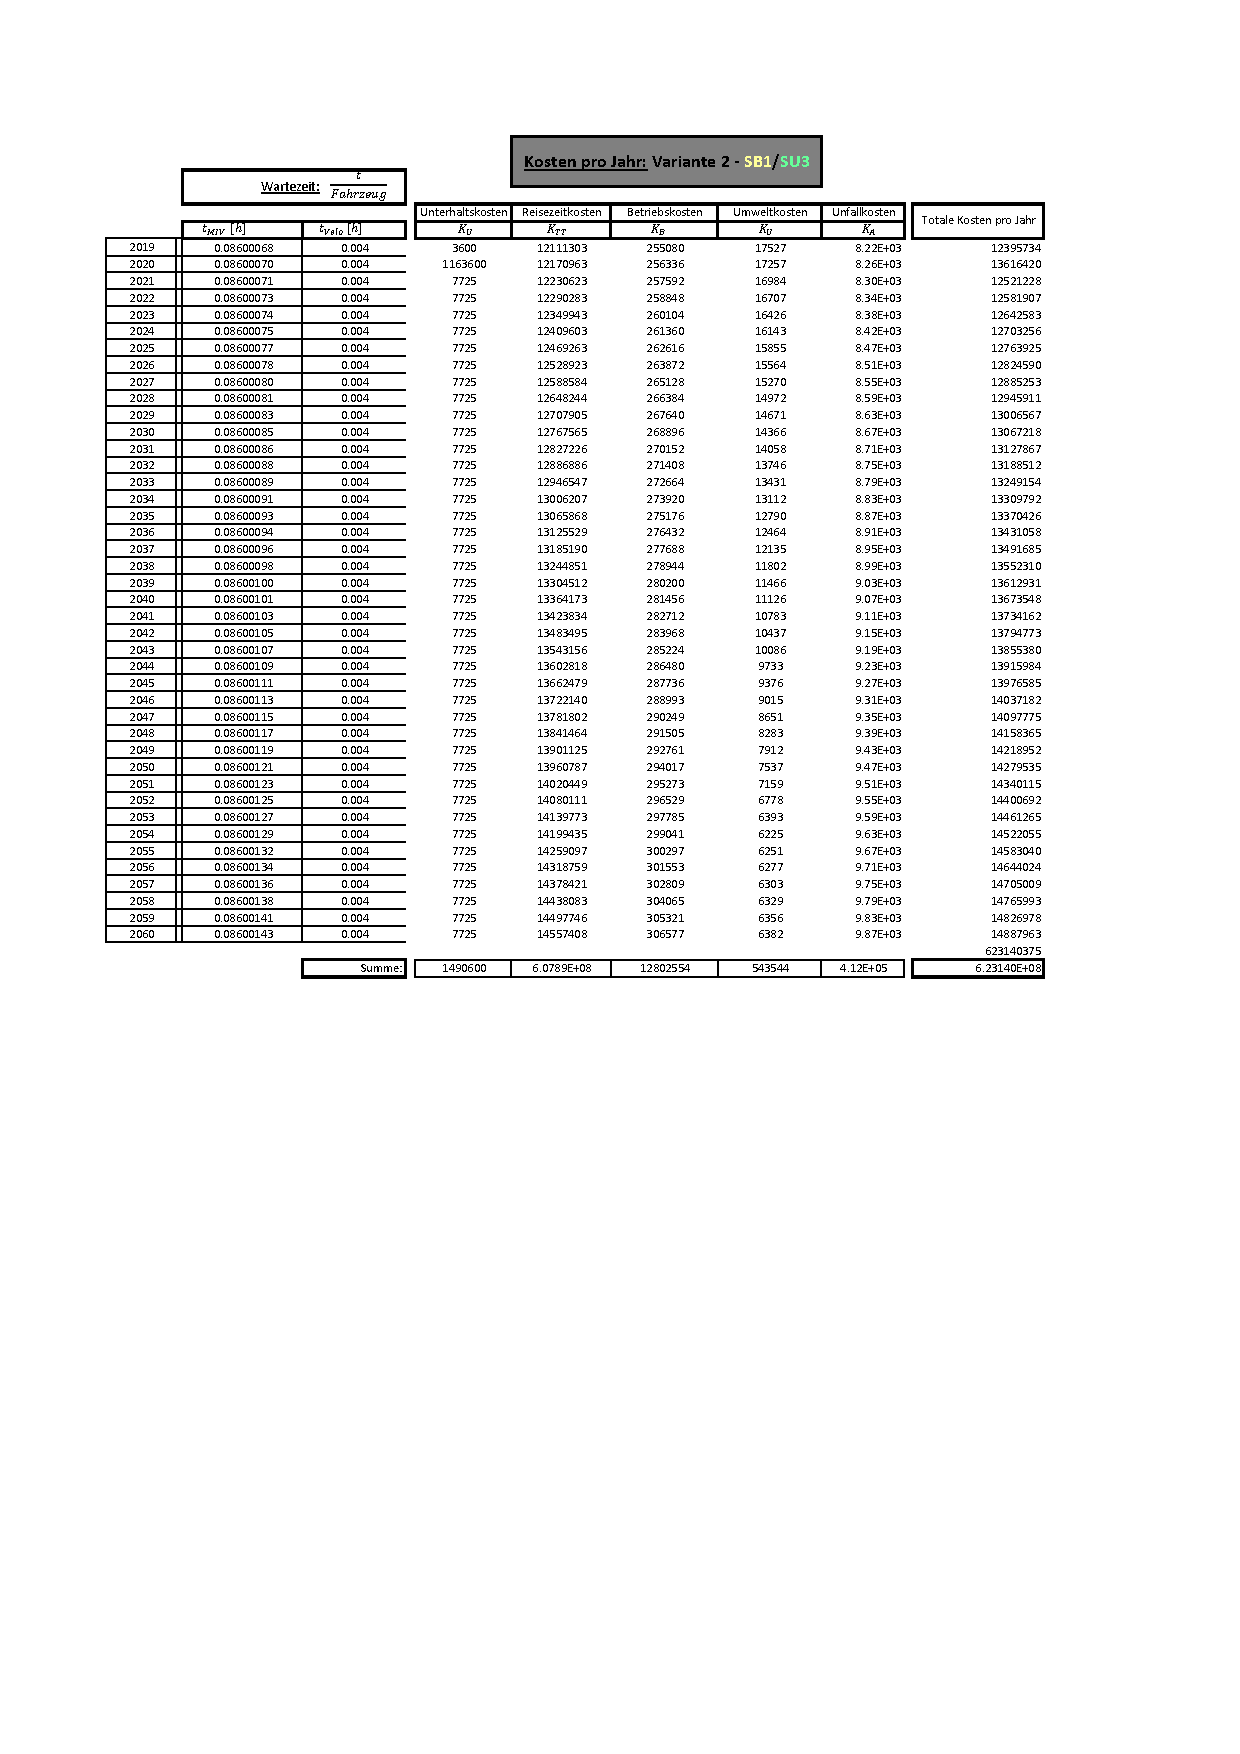
\includegraphics[width=\textwidth]{figures/Anhang/f-00-A-V2-B1-U3}
	\caption{Kostenberechung Variante 2 - SB1/SU3}
\end{figure}

\begin{figure}[h!]
	\centering
	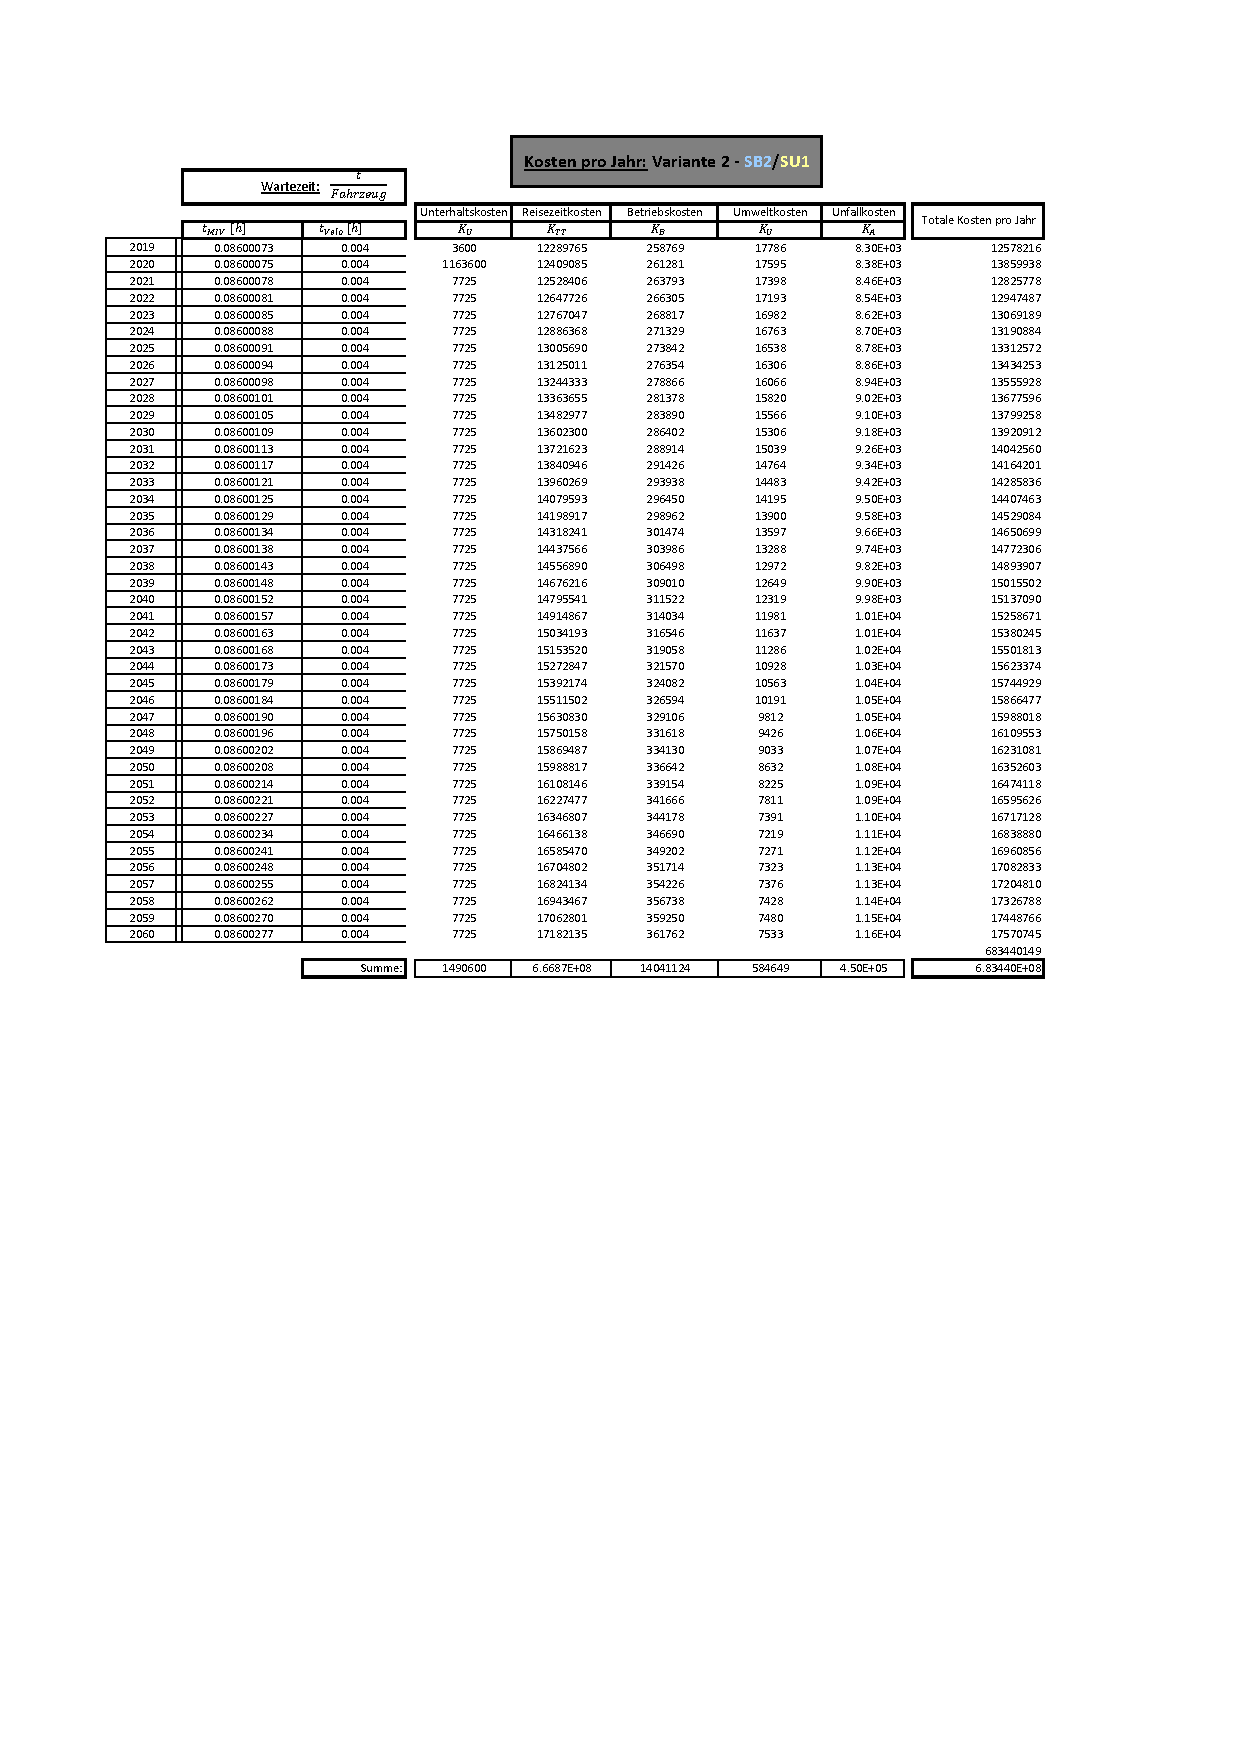
\includegraphics[width=\textwidth]{figures/Anhang/f-00-A-V2-B2-U1}
	\caption{Kostenberechung Variante 2 - SB2/SU1}
\end{figure}

\begin{figure}[h!]
	\centering
	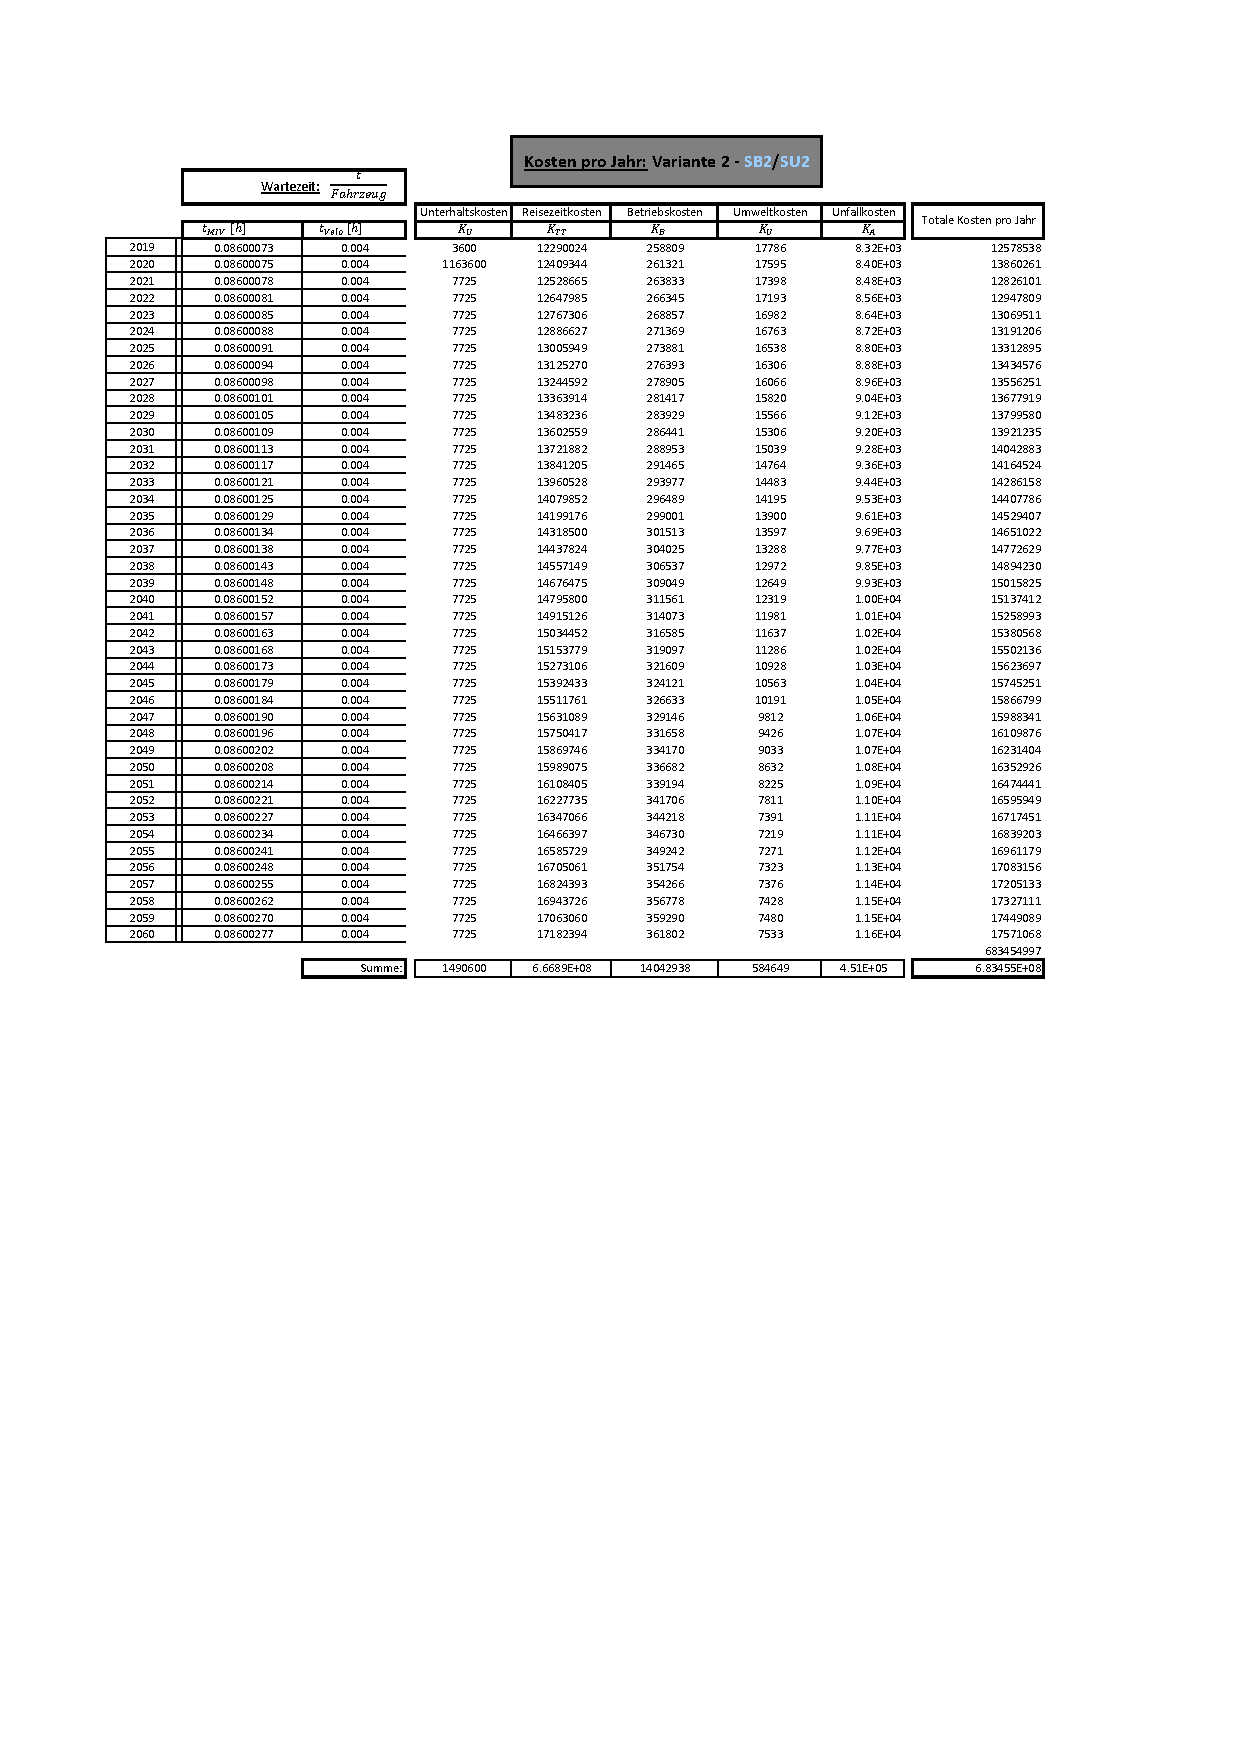
\includegraphics[width=\textwidth]{figures/Anhang/f-00-A-V2-B2-U2}
	\caption{Kostenberechung Variante 2 - SB2/SU2}
\end{figure}

\begin{figure}[h!]
	\centering
	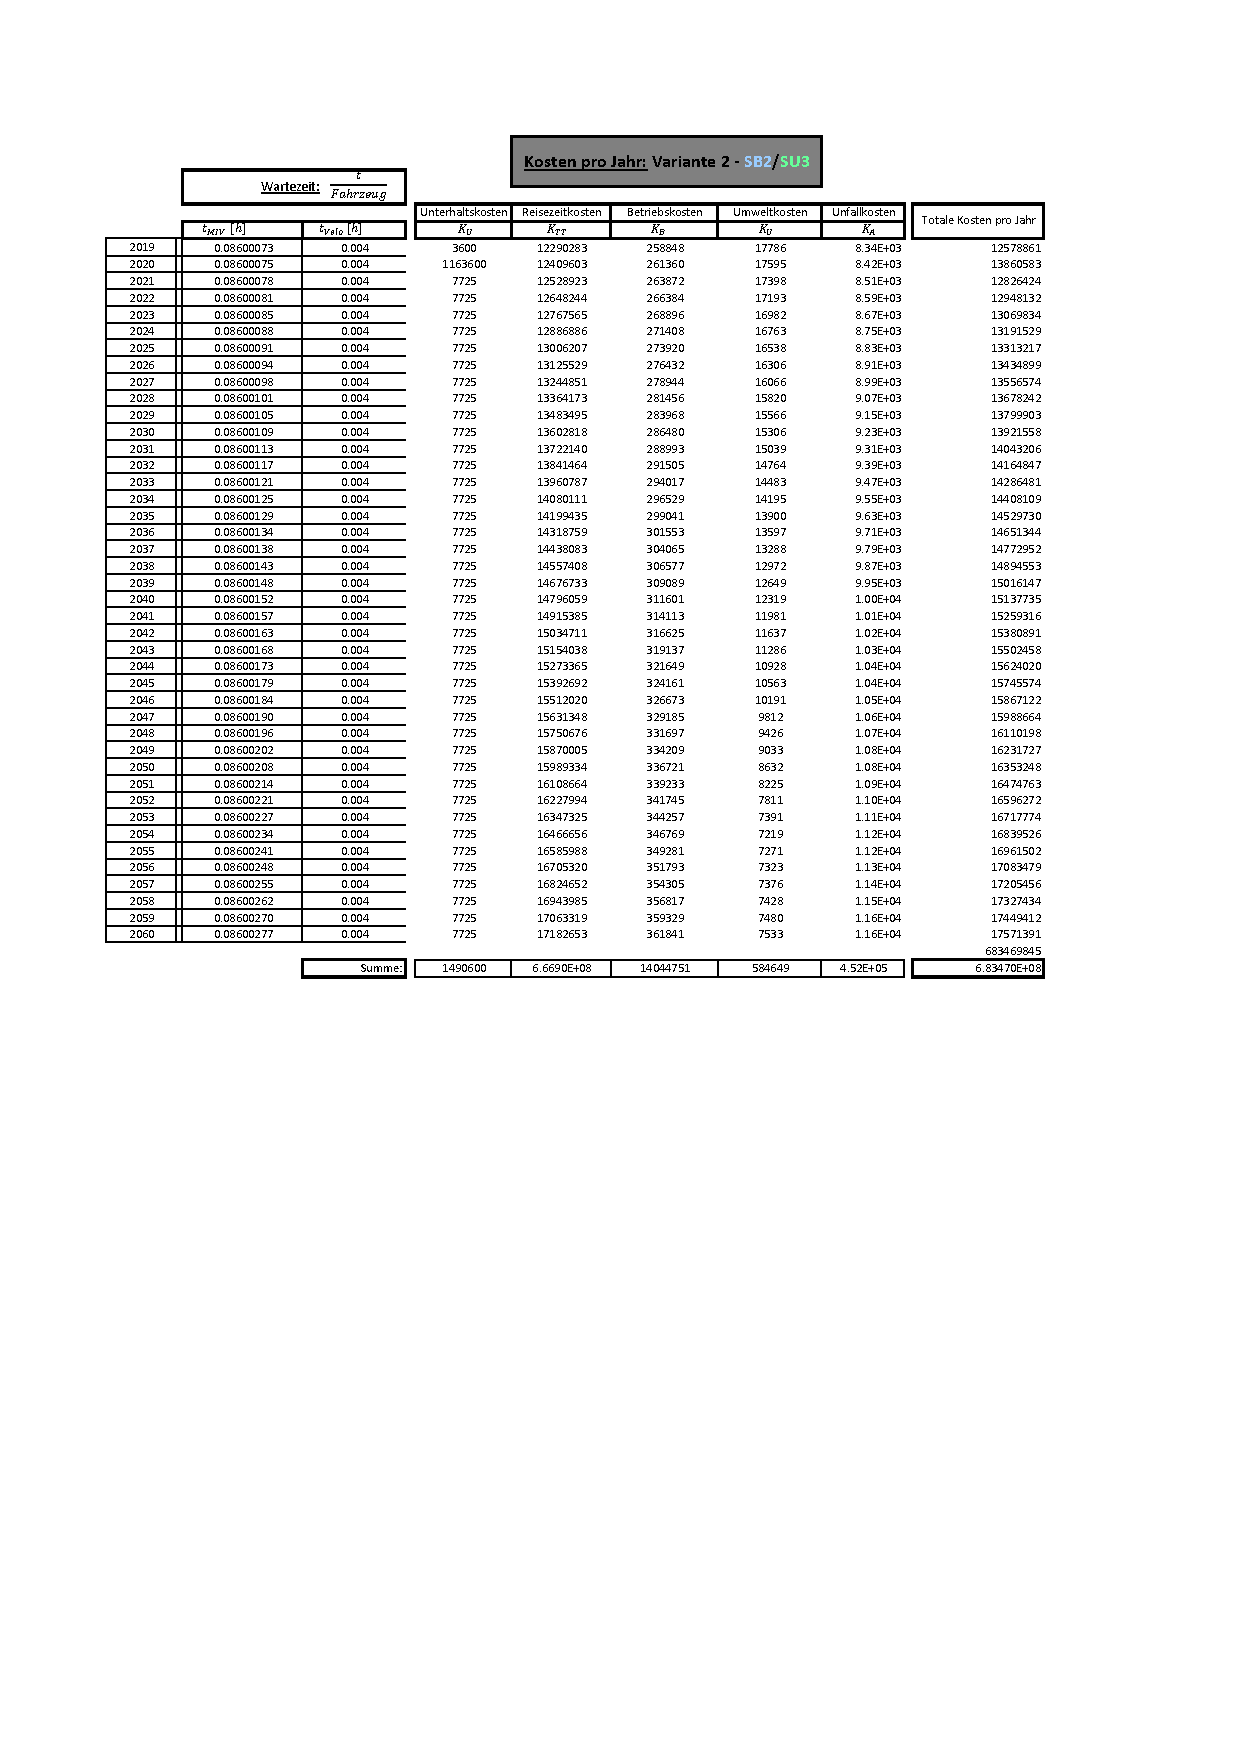
\includegraphics[width=\textwidth]{figures/Anhang/f-00-A-V2-B2-U3}
	\caption{Kostenberechung Variante 2 - SB2/SU3}
\end{figure}

\begin{figure}[h!]
	\centering
	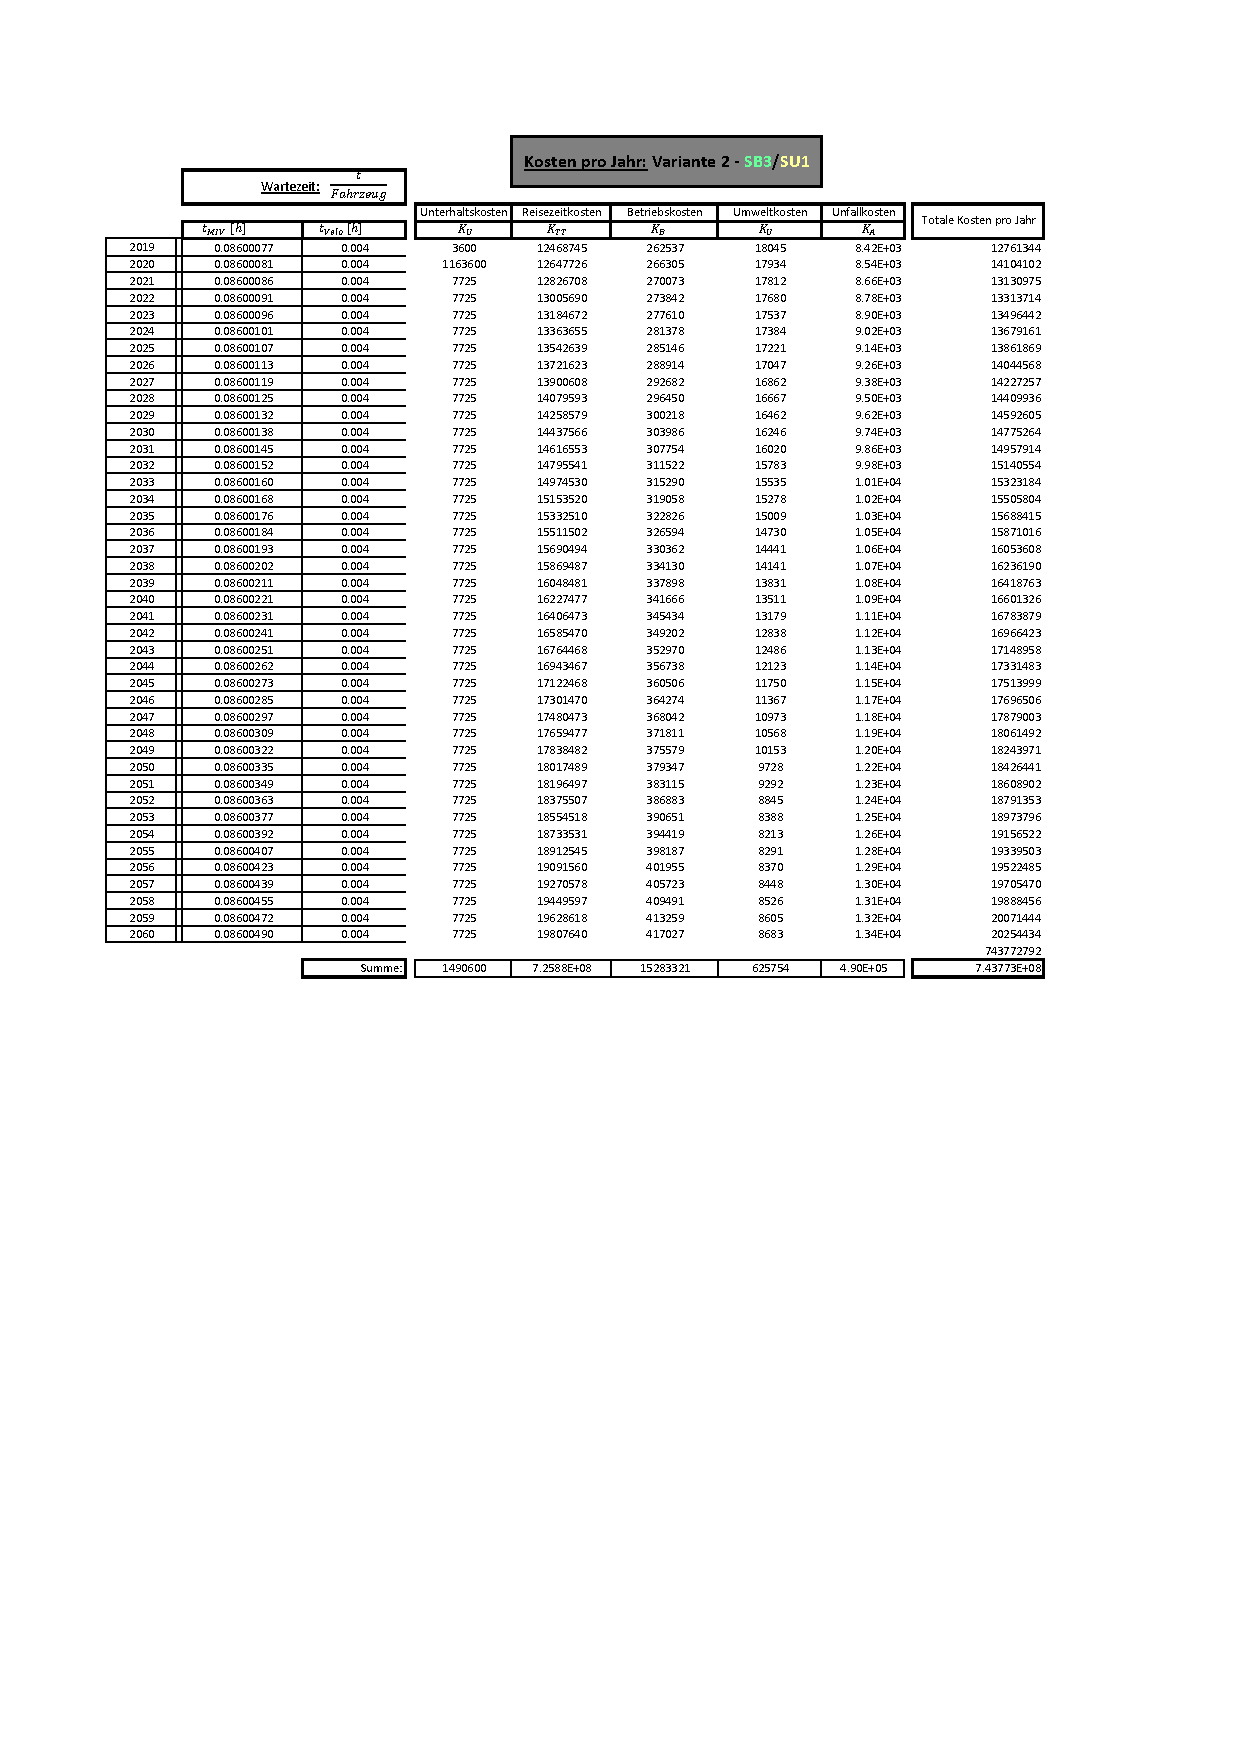
\includegraphics[width=\textwidth]{figures/Anhang/f-00-A-V2-B3-U1}
	\caption{Kostenberechung Variante 2 - SB3/SU1}
\end{figure}

\begin{figure}[h!]
	\centering
	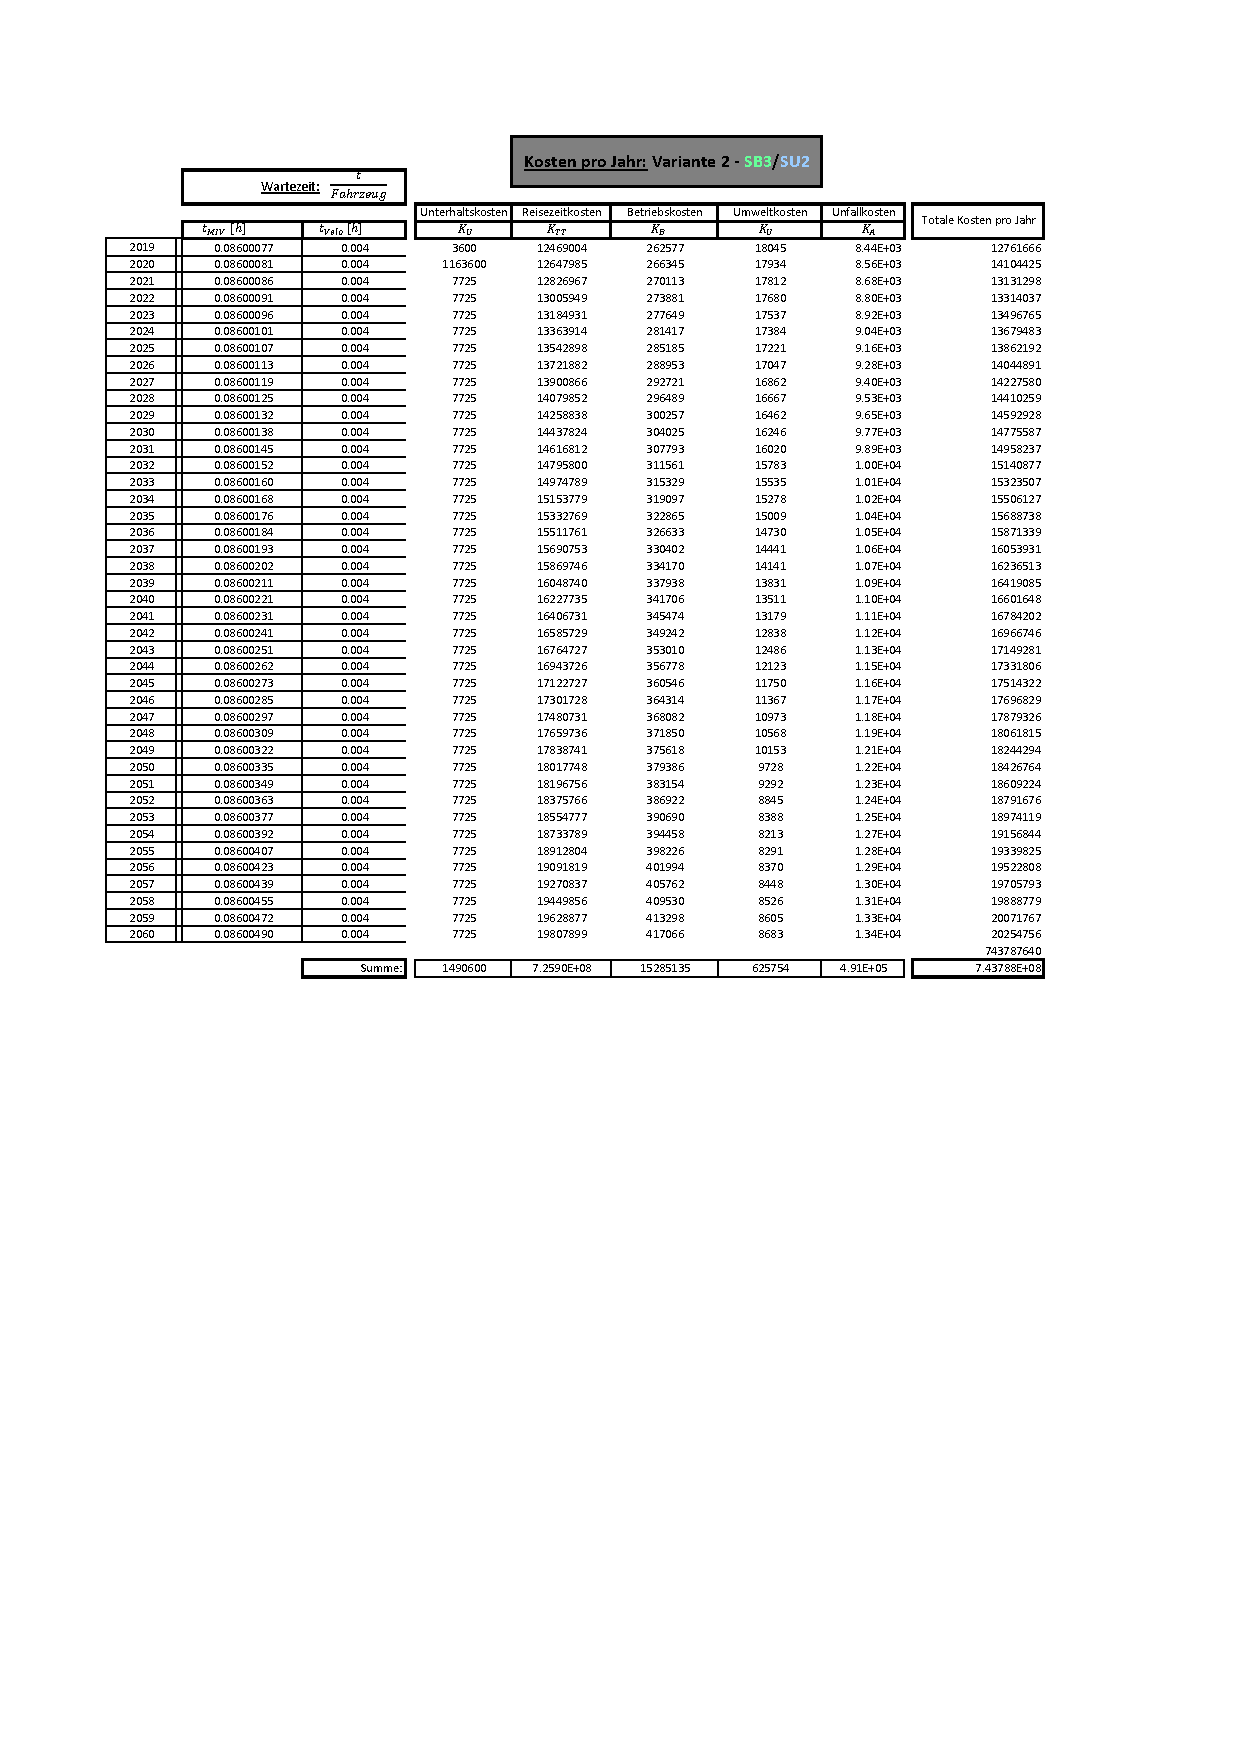
\includegraphics[width=\textwidth]{figures/Anhang/f-00-A-V2-B3-U2}
	\caption{Kostenberechung Variante 2 - SB3/SU2}
\end{figure}

\begin{figure}[h!]
	\centering
	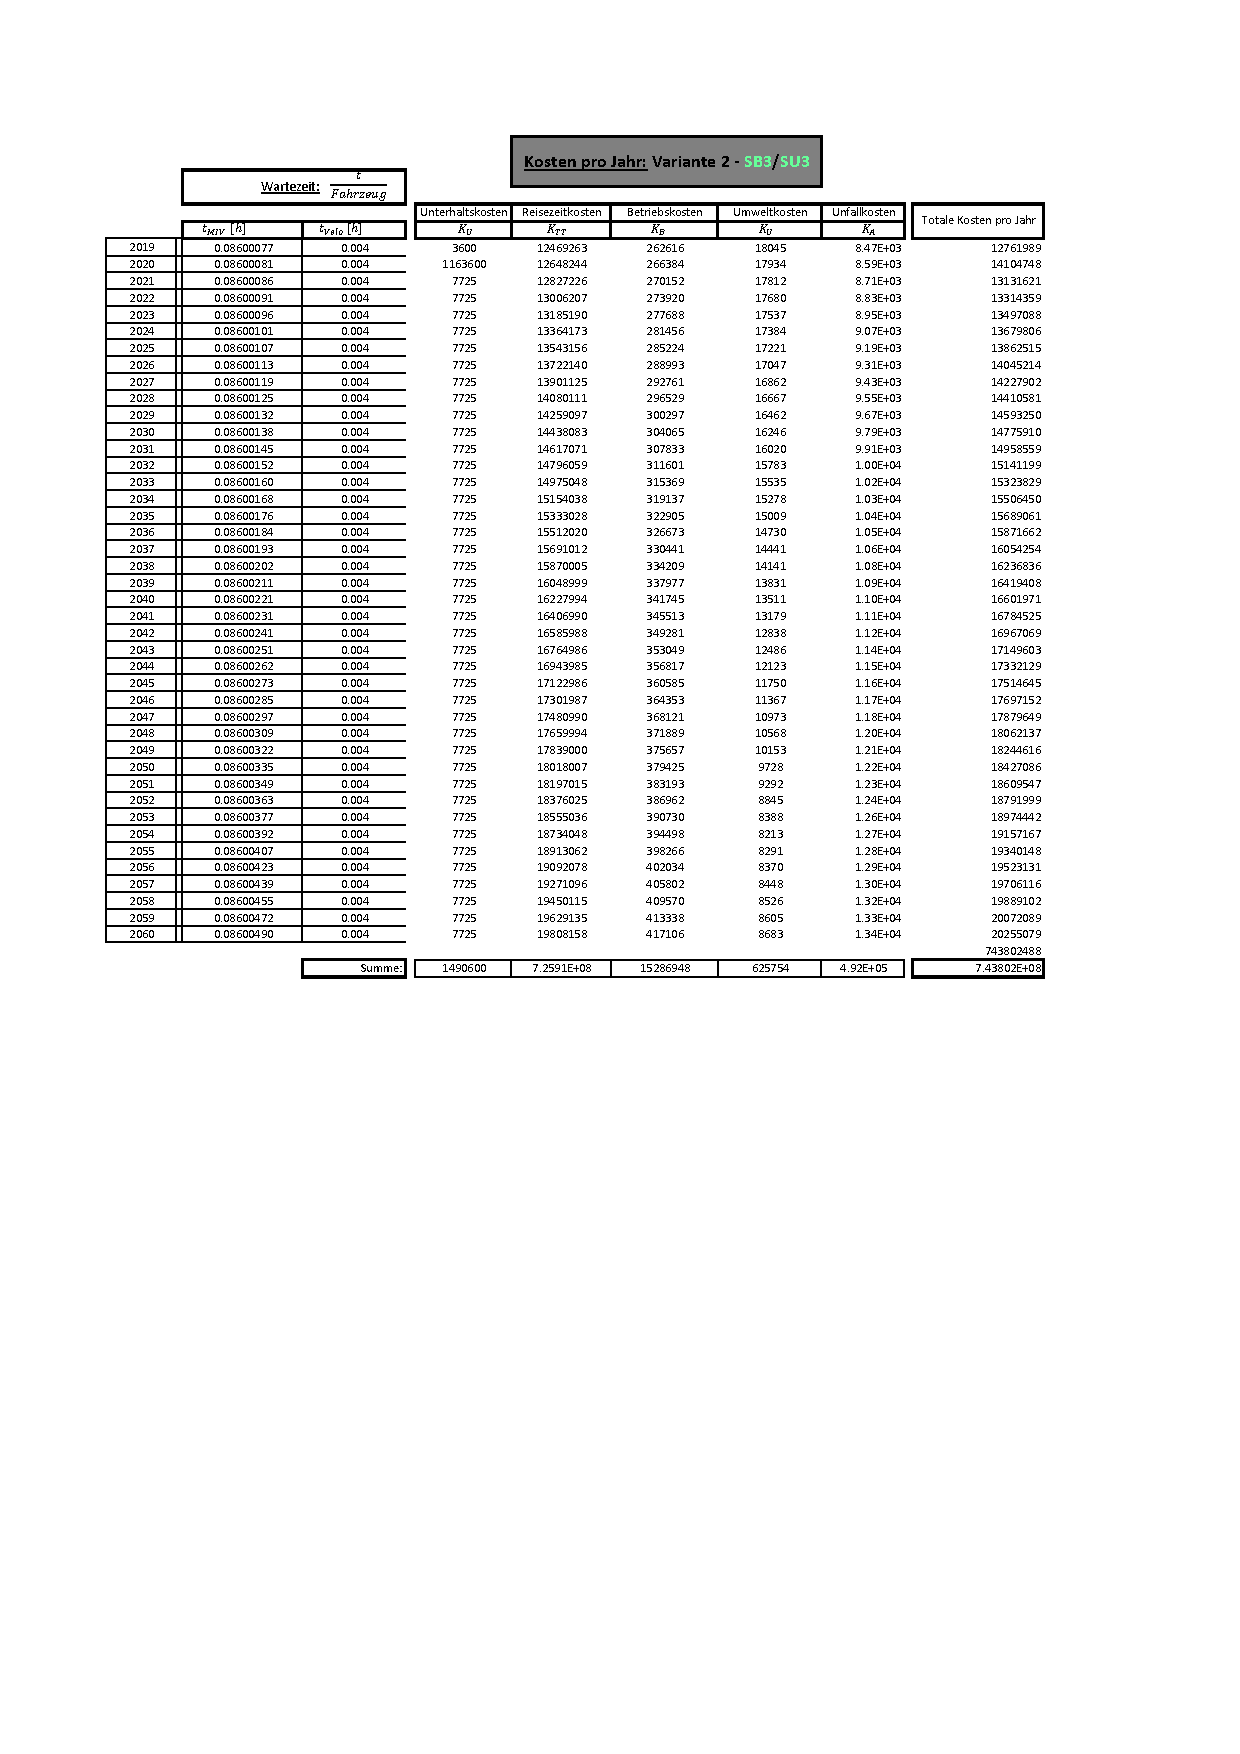
\includegraphics[width=\textwidth]{figures/Anhang/f-00-A-V2-B3-U3}
	\caption{Kostenberechung Variante 2 - SB3/SU3}
\end{figure}

\begin{figure}[h!]
	\centering
	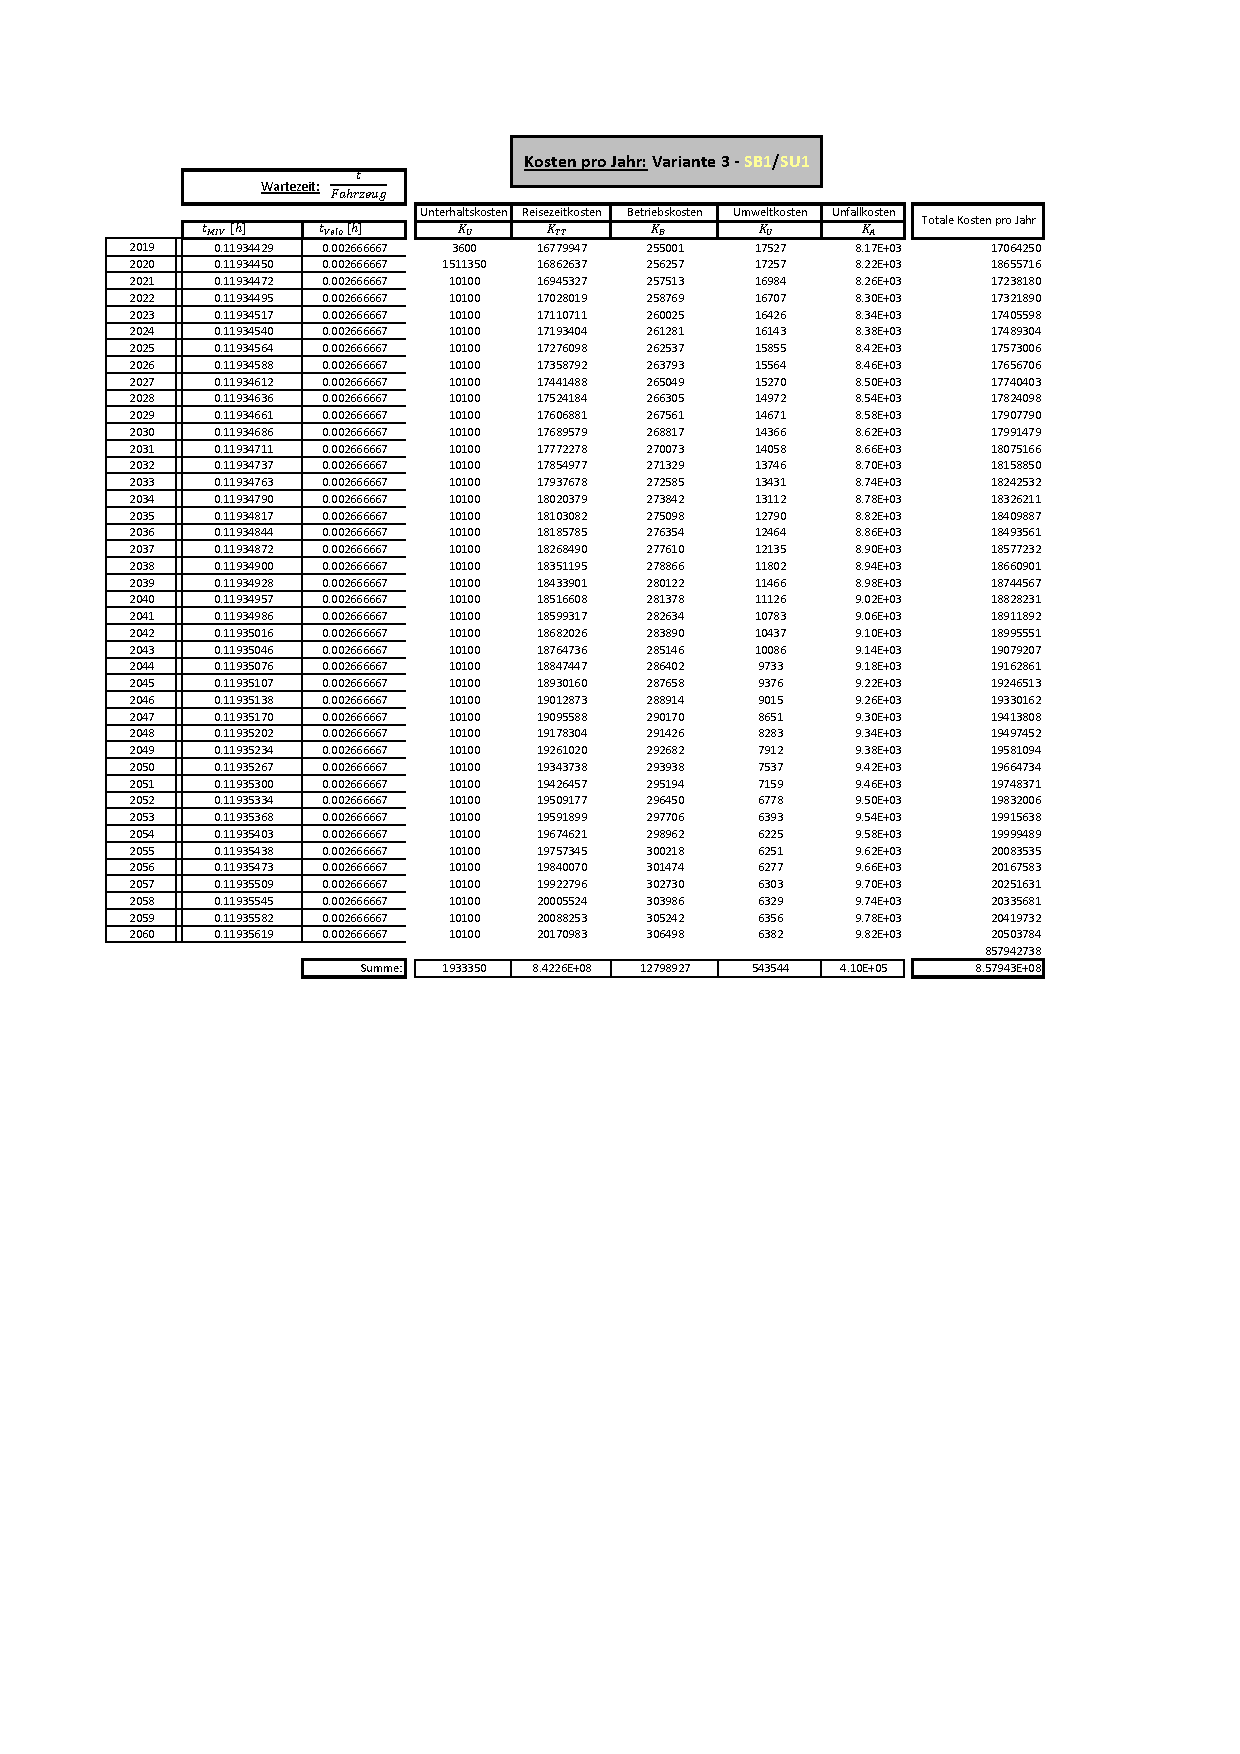
\includegraphics[width=\textwidth]{figures/Anhang/f-00-A-V3-B1-U1}
	\caption{Kostenberechung Variante 3 - SB1/SU1}
\end{figure}

\begin{figure}[h!]
	\centering
	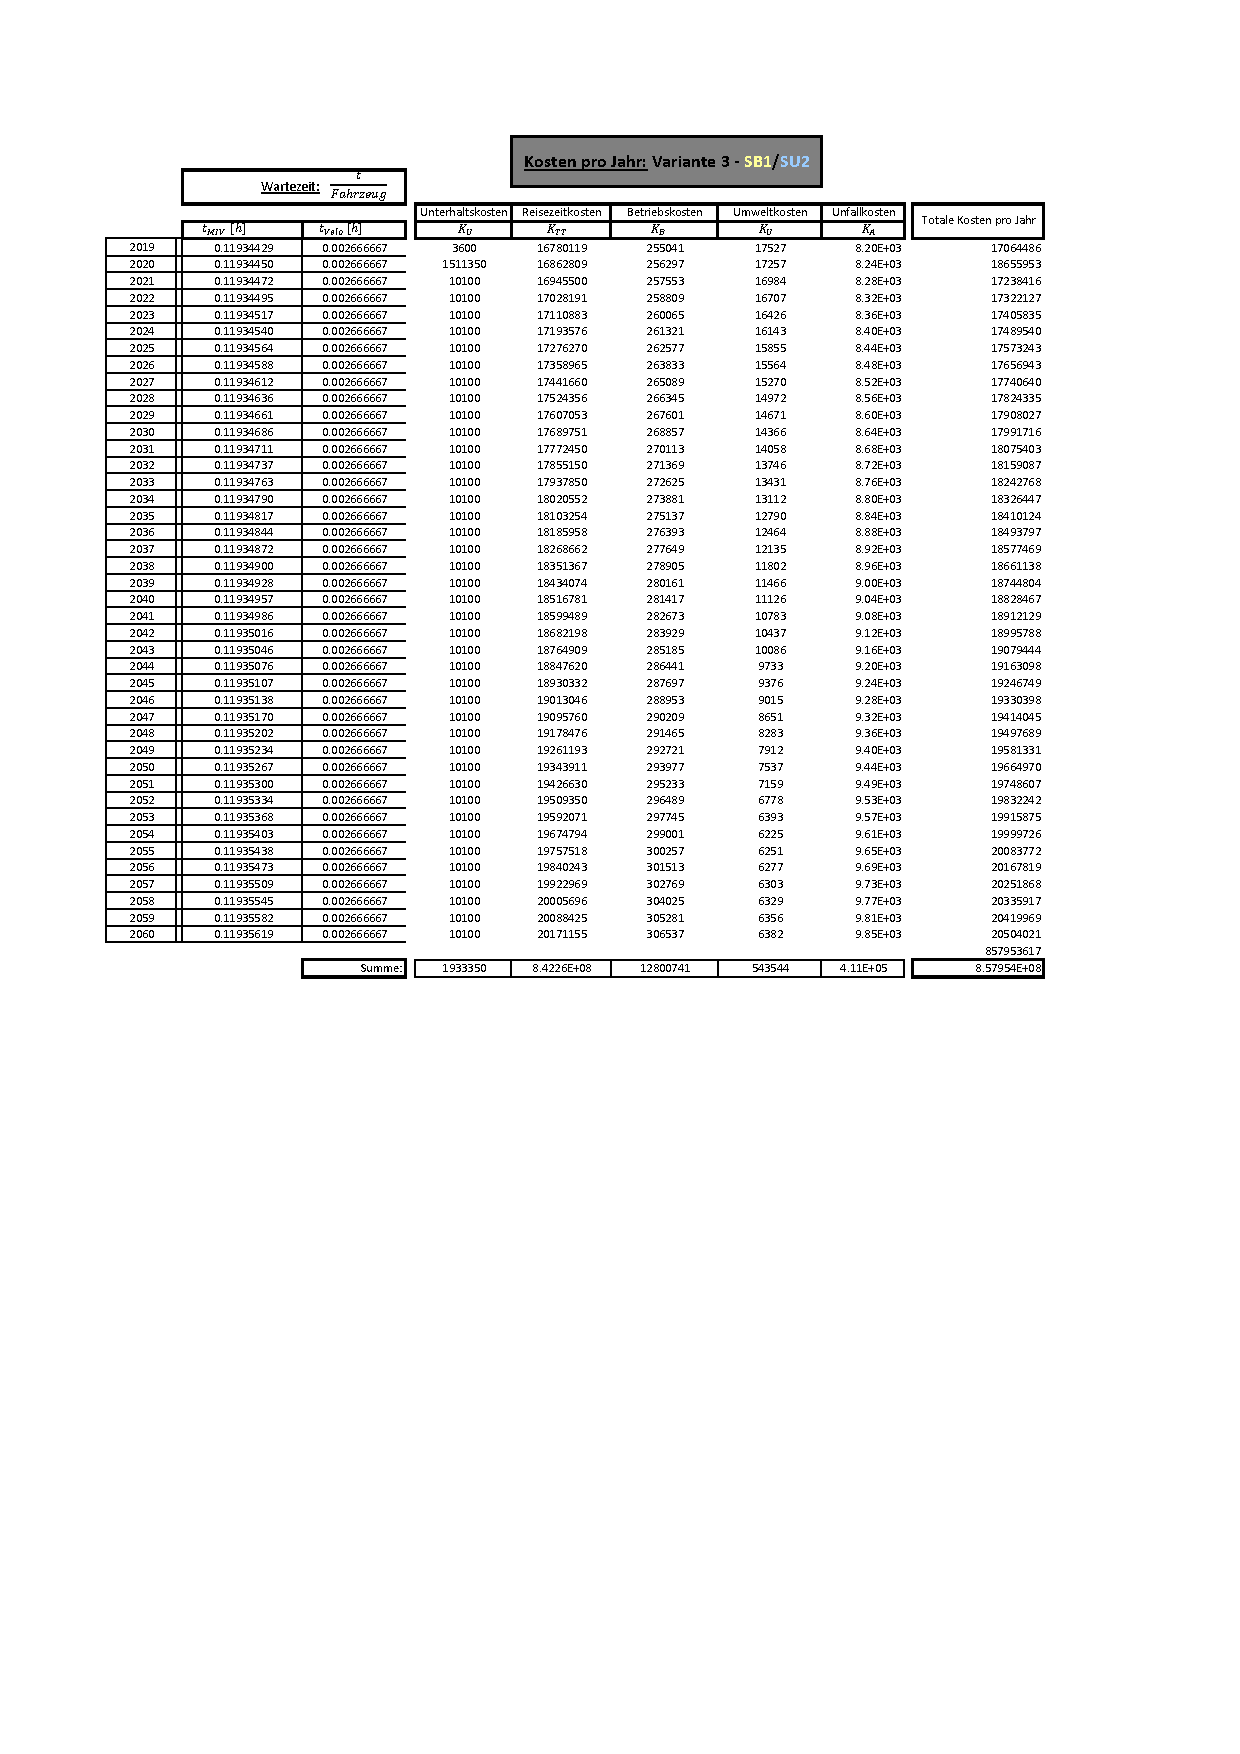
\includegraphics[width=\textwidth]{figures/Anhang/f-00-A-V3-B1-U2}
	\caption{Kostenberechung Variante 3 - SB1/SU2}
\end{figure}

\begin{figure}[h!]
	\centering
	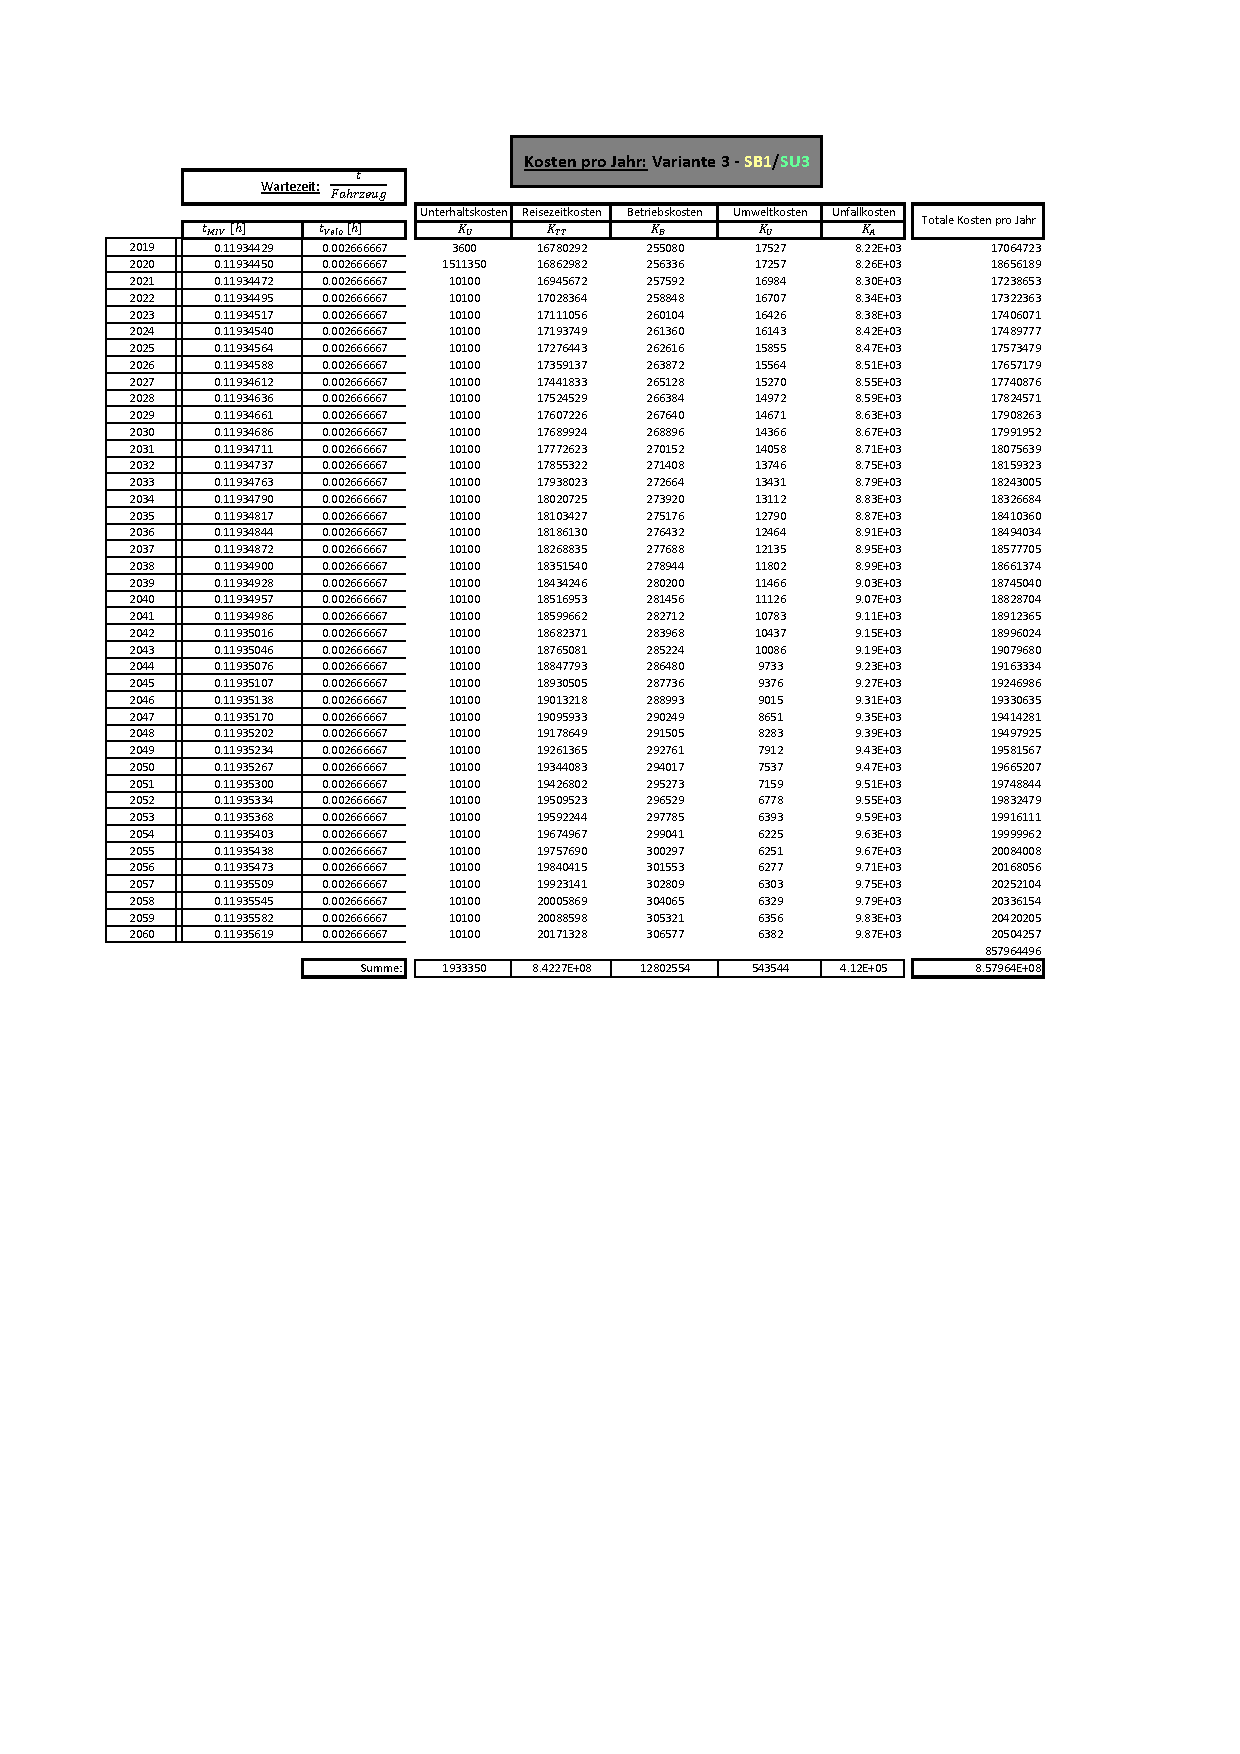
\includegraphics[width=\textwidth]{figures/Anhang/f-00-A-V3-B1-U3}
	\caption{Kostenberechung Variante 3 - SB1/SU3}
\end{figure}

\begin{figure}[h!]
	\centering
	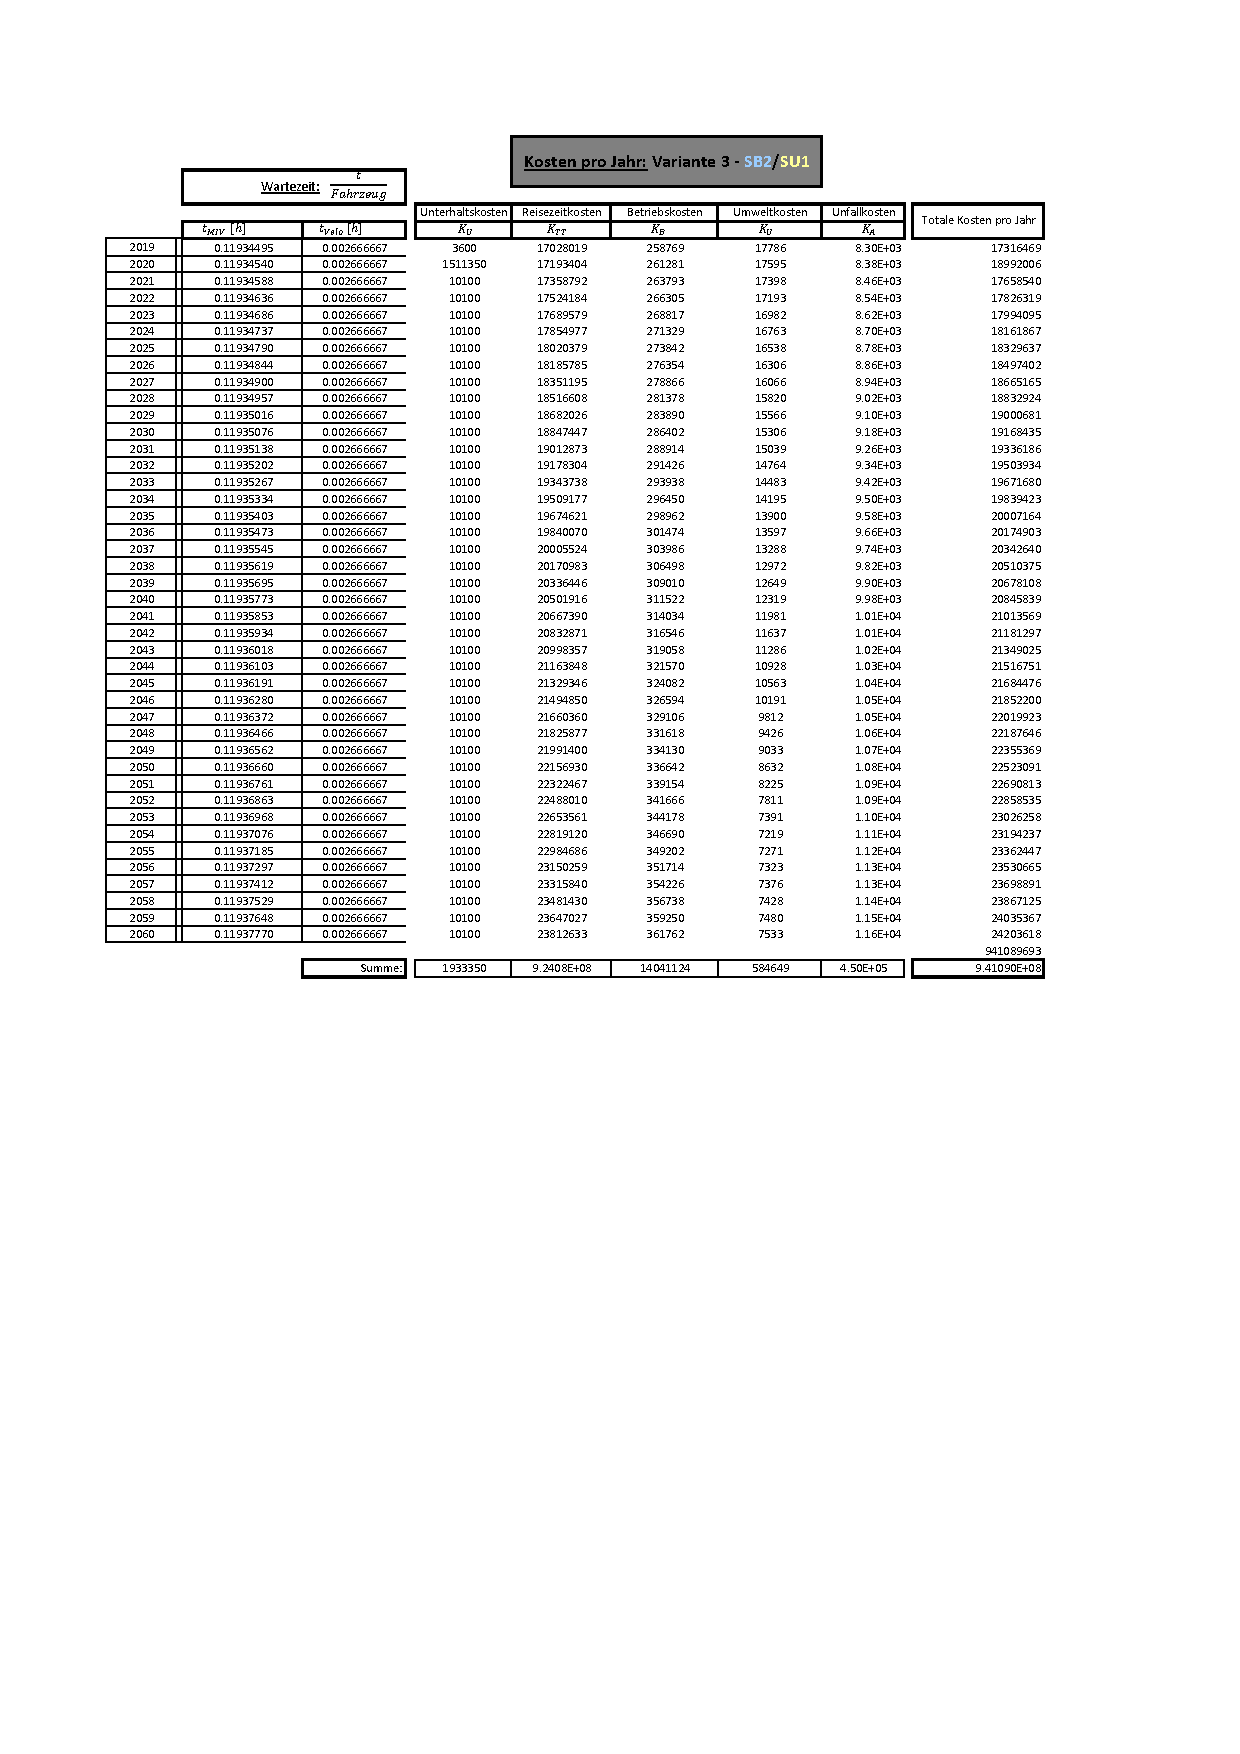
\includegraphics[width=\textwidth]{figures/Anhang/f-00-A-V3-B2-U1}
	\caption{Kostenberechung Variante 3 - SB2/SU1}
\end{figure}

\begin{figure}[h!]
	\centering
	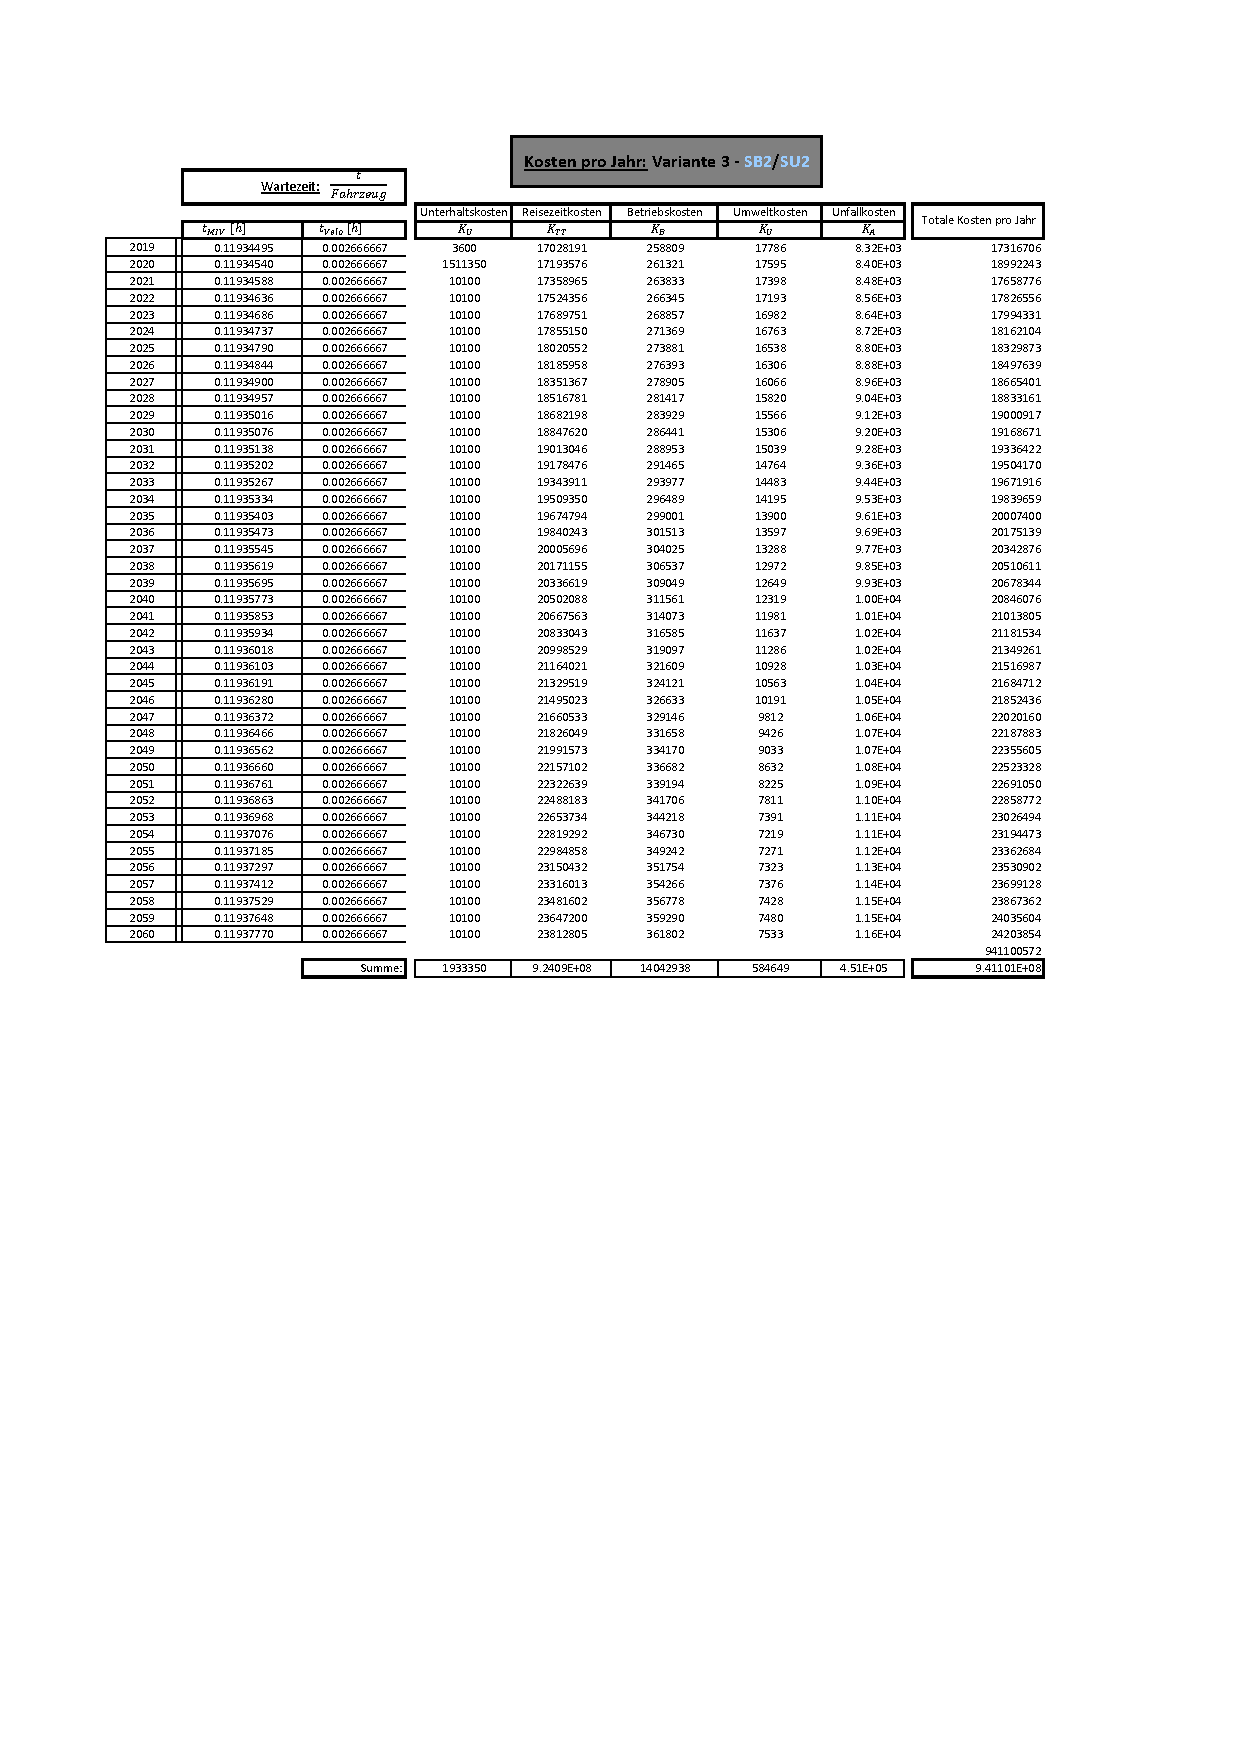
\includegraphics[width=\textwidth]{figures/Anhang/f-00-A-V3-B2-U2}
	\caption{Kostenberechung Variante 3 - SB2/SU2}
\end{figure}

\begin{figure}[h!]
	\centering
	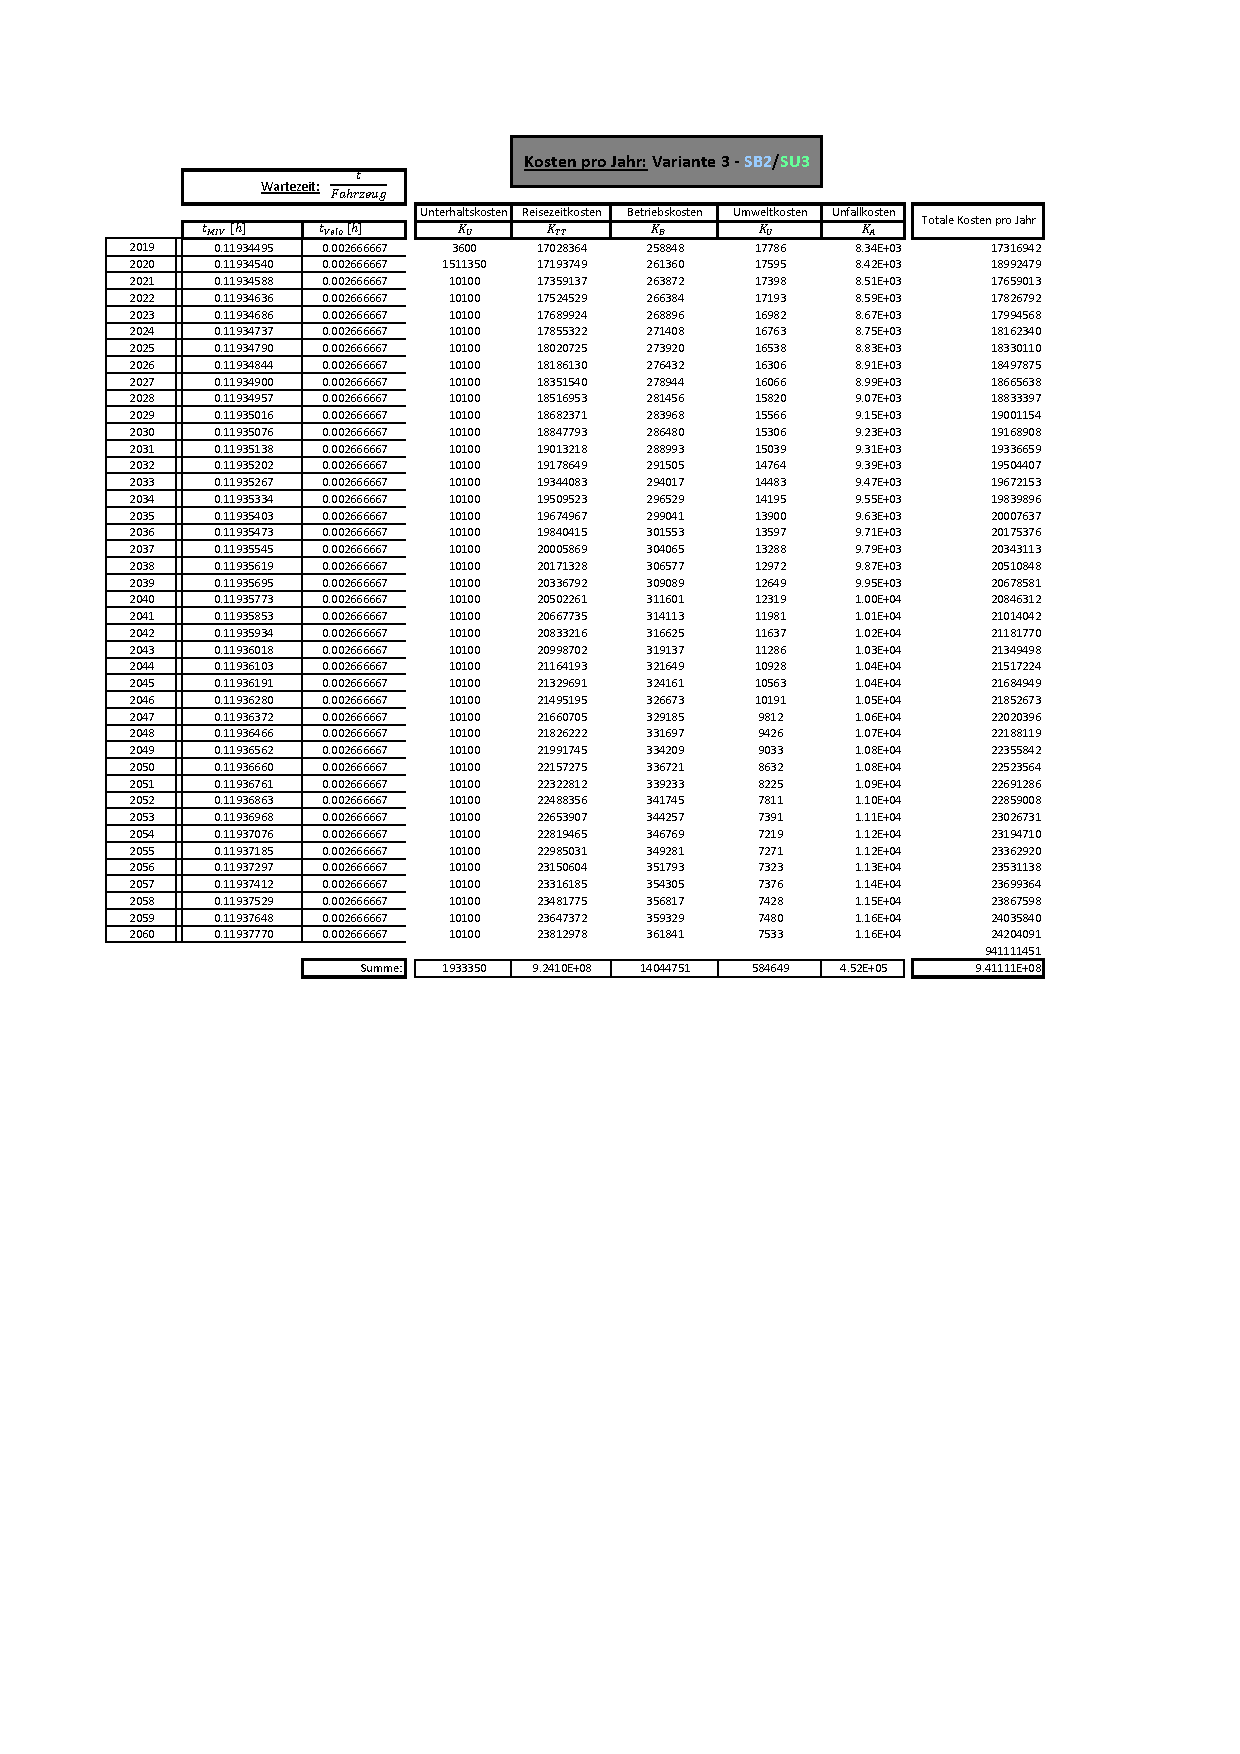
\includegraphics[width=\textwidth]{figures/Anhang/f-00-A-V3-B2-U3}
	\caption{Kostenberechung Variante 3 - SB2/SU3}
\end{figure}

\begin{figure}[h!]
	\centering
	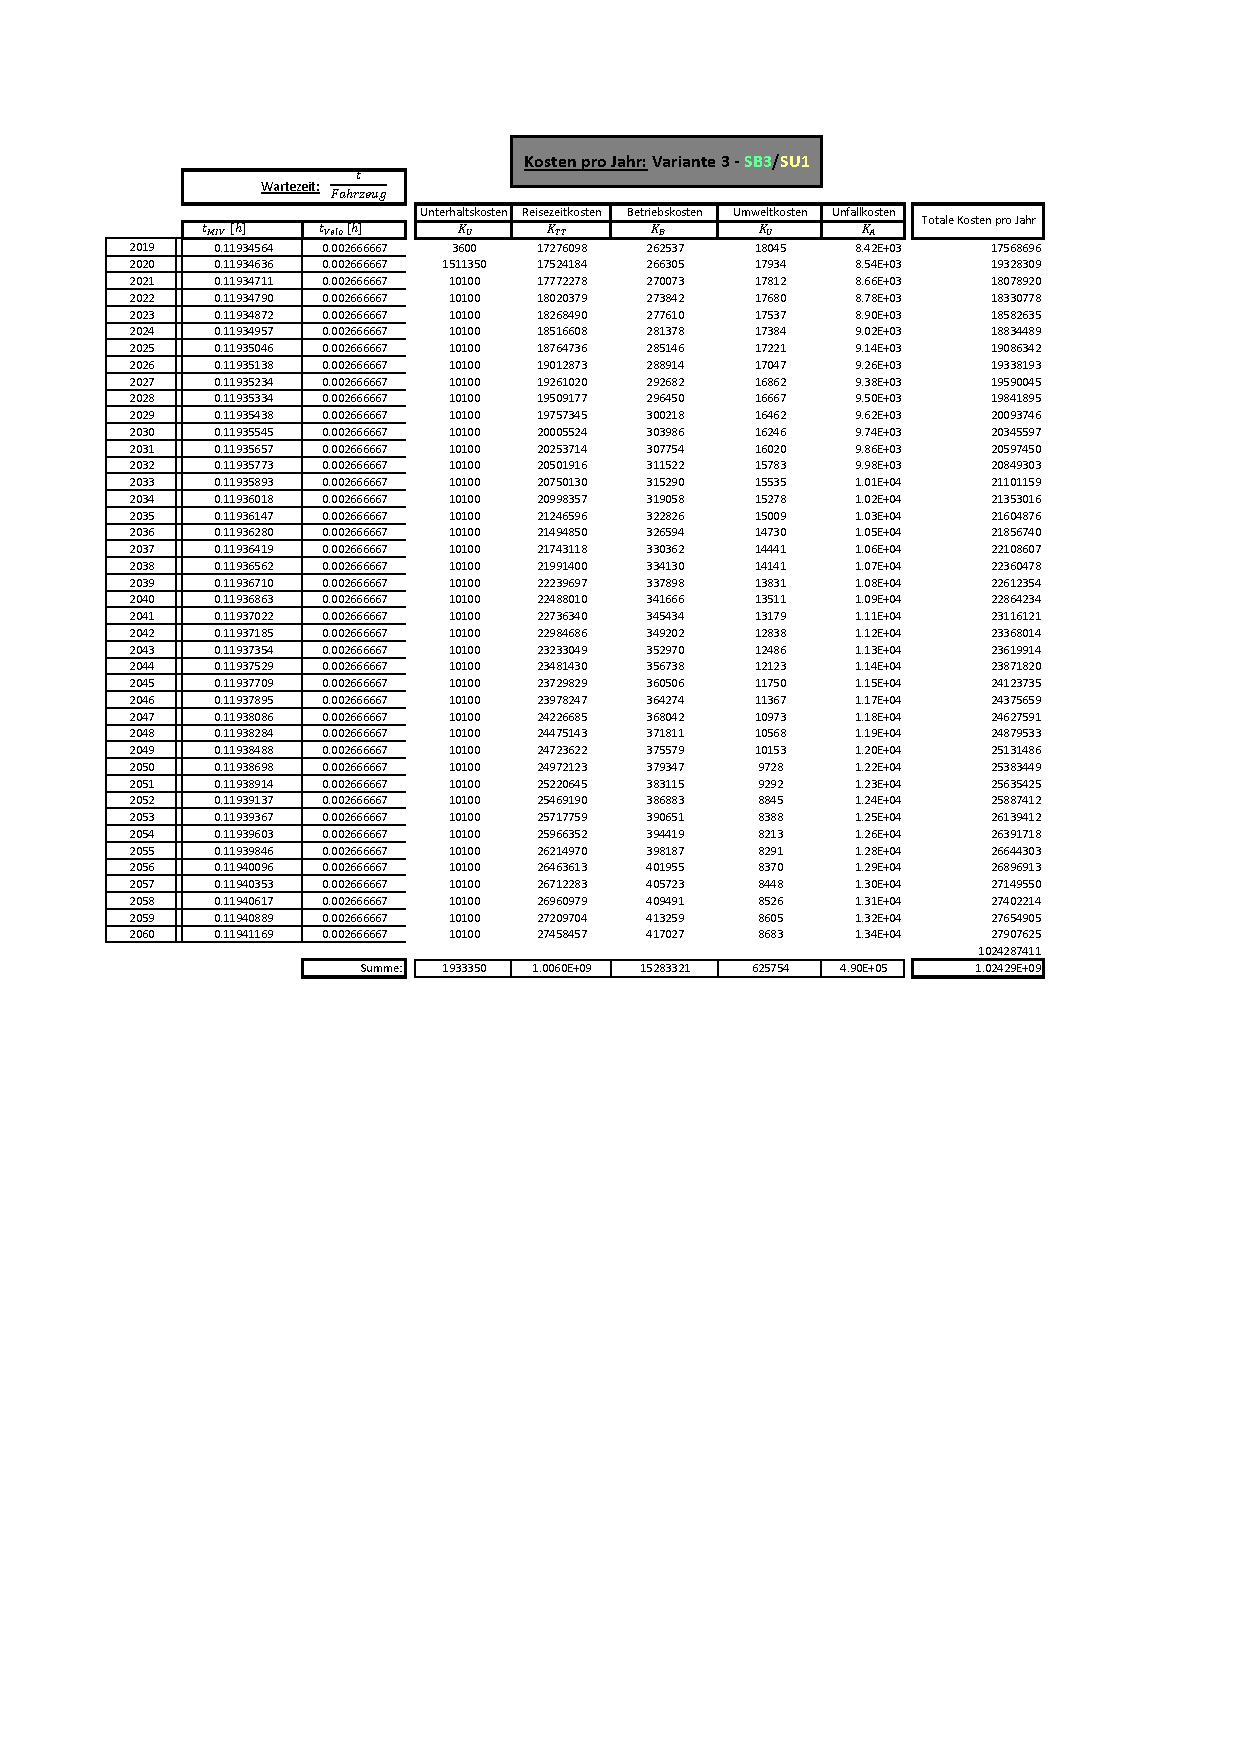
\includegraphics[width=\textwidth]{figures/Anhang/f-00-A-V3-B3-U1}
	\caption{Kostenberechung Variante 3 - SB3/SU1}
\end{figure}

\begin{figure}[h!]
	\centering
	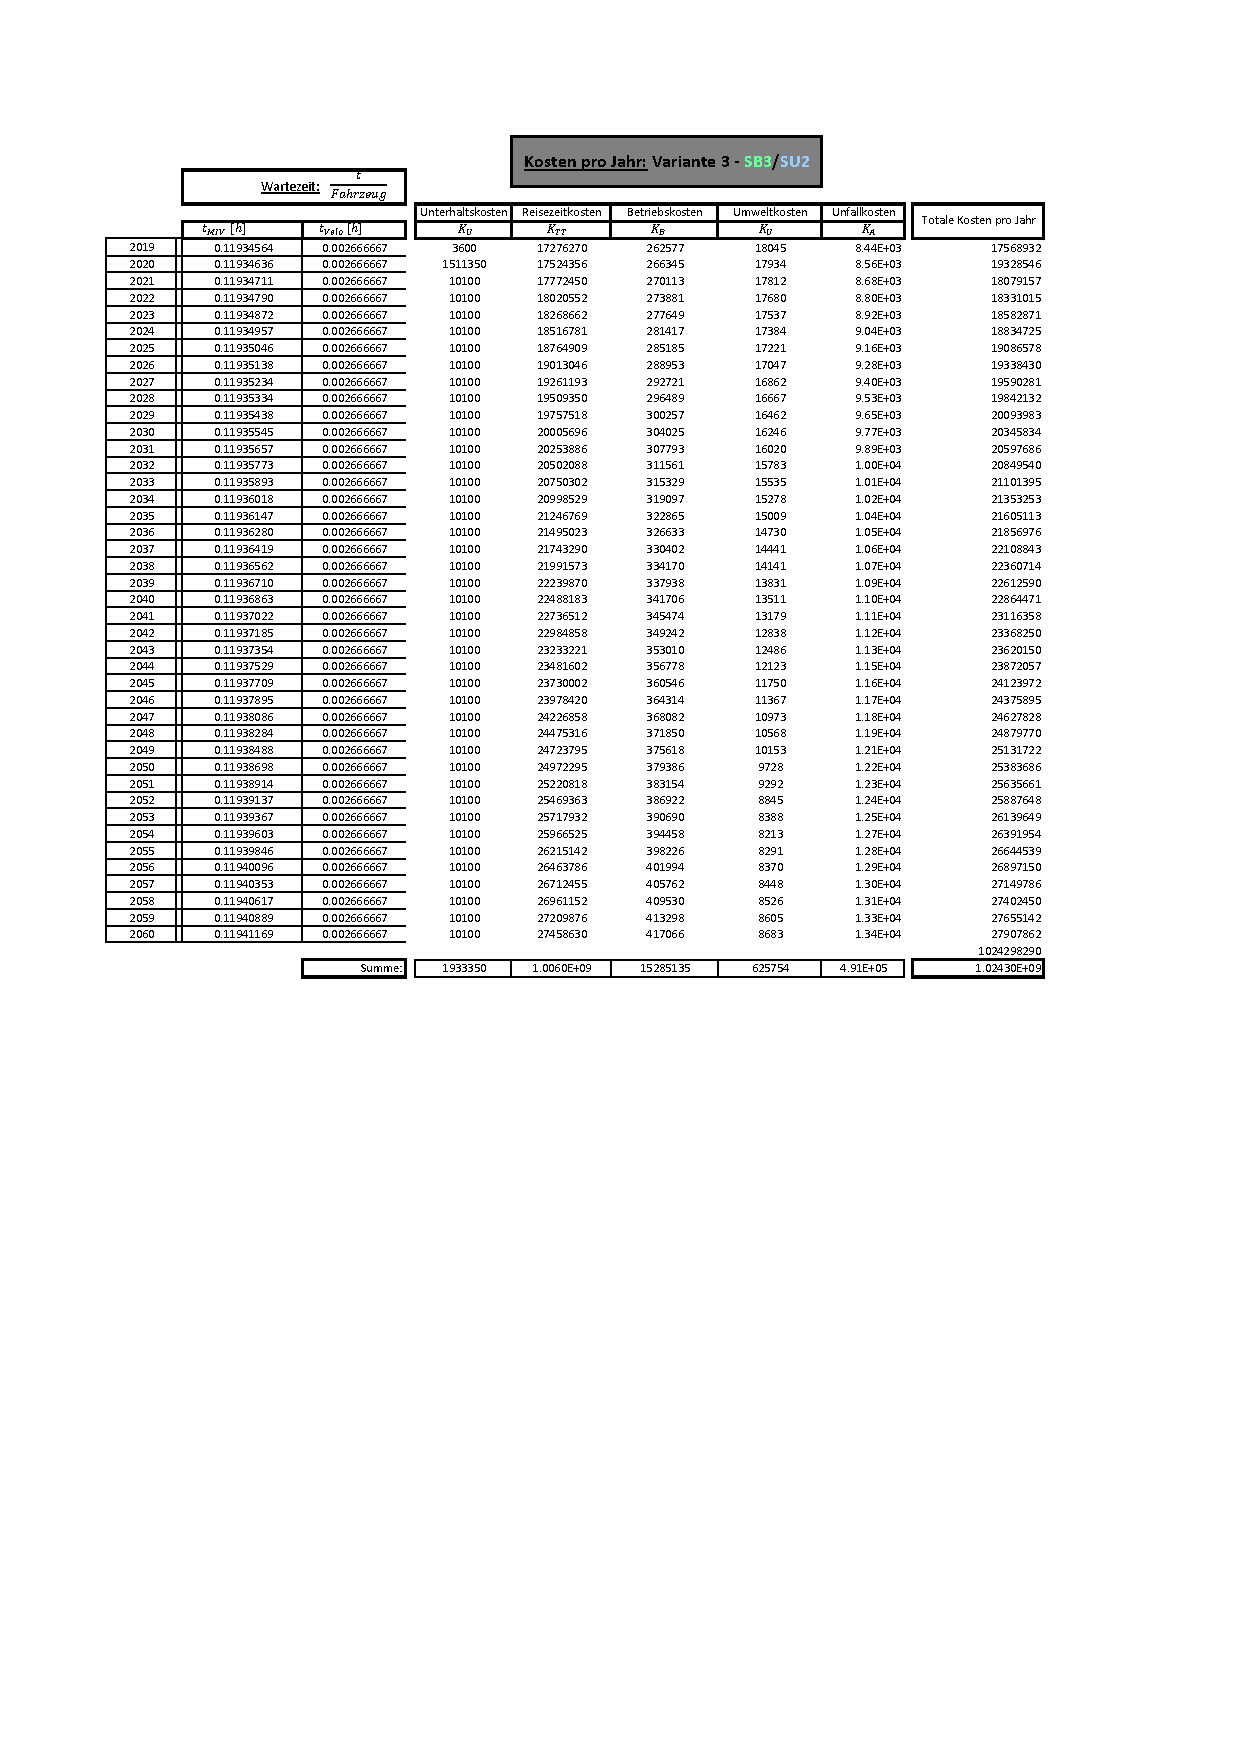
\includegraphics[width=\textwidth]{figures/Anhang/f-00-A-V3-B3-U2}
	\caption{Kostenberechung Variante 3 - SB3/SU2}
\end{figure}

\begin{figure}[h!]
	\centering
	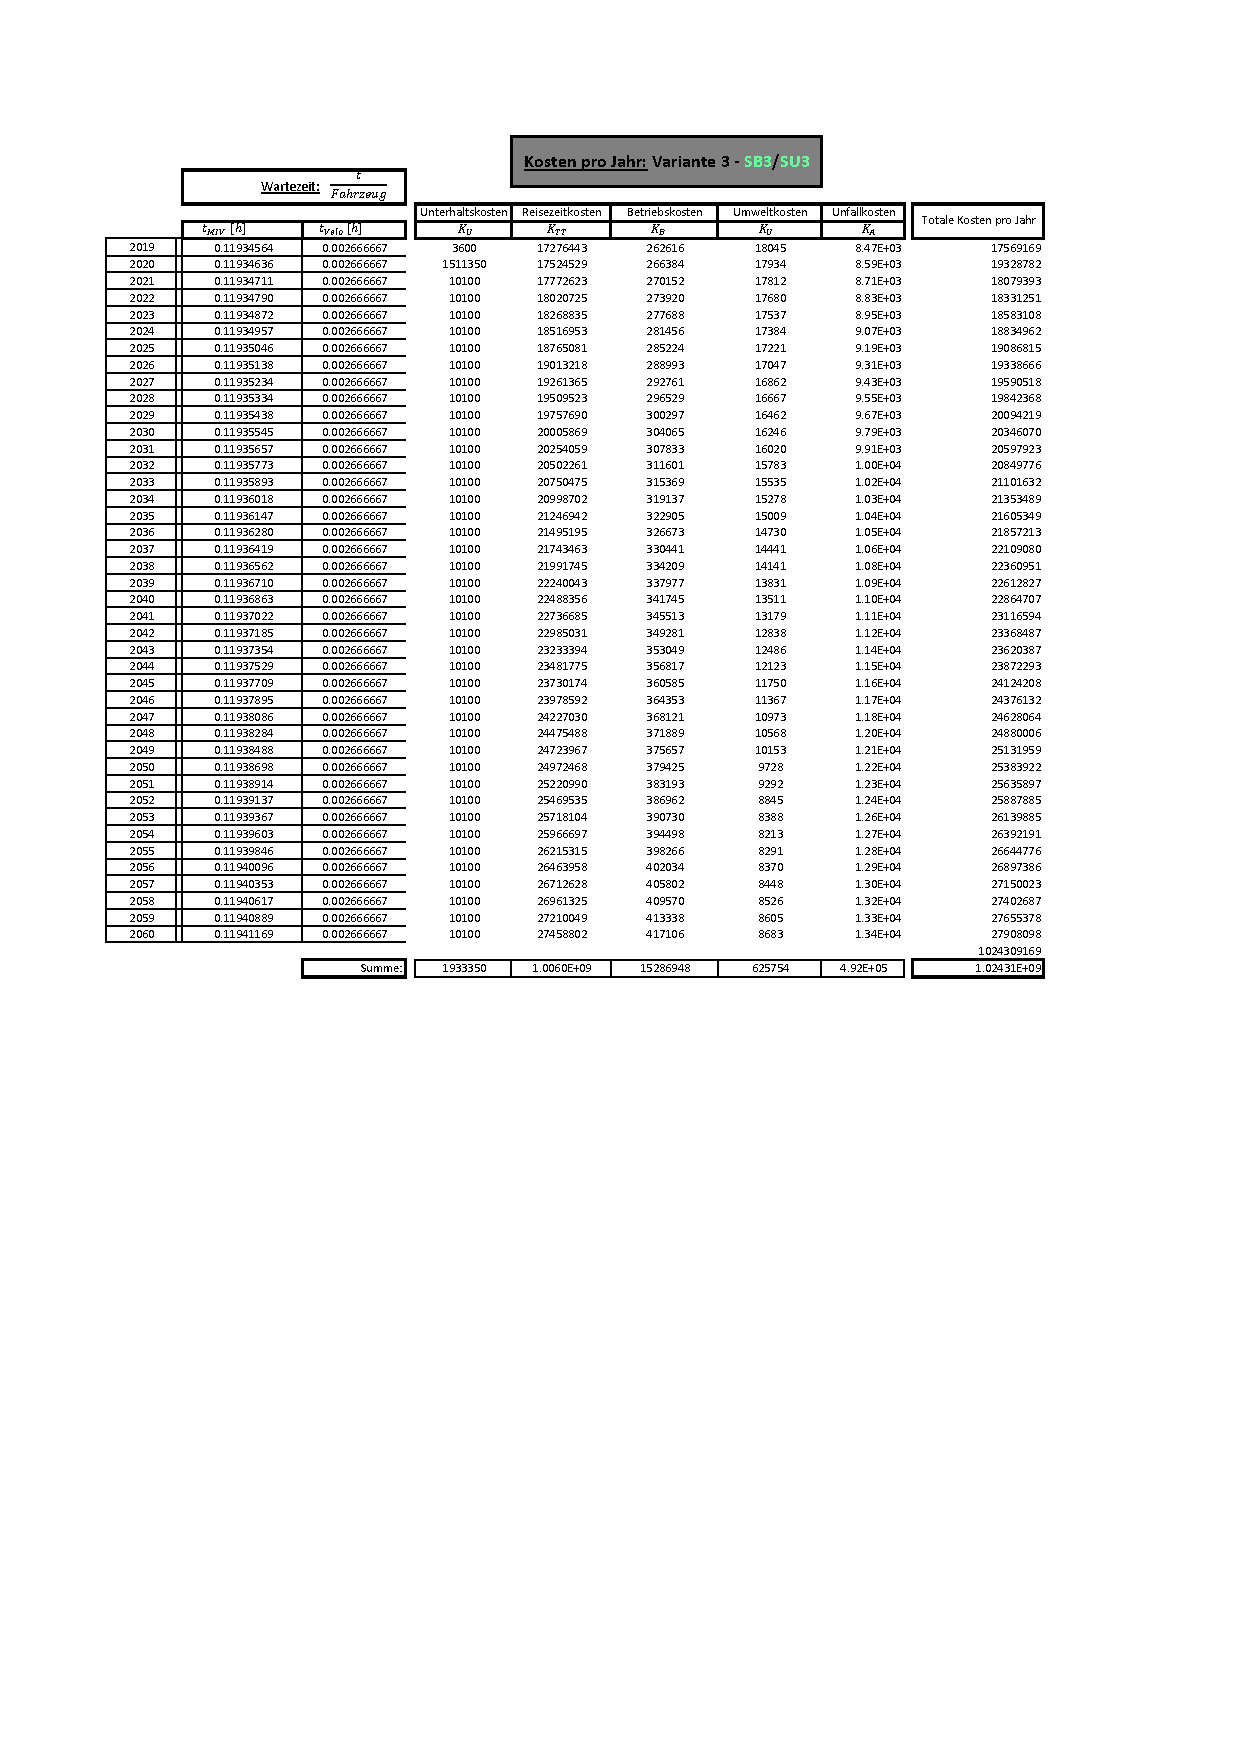
\includegraphics[width=\textwidth]{figures/Anhang/f-00-A-V3-B3-U3}
	\caption{Kostenberechung Variante 3 - SB3/SU3}
\end{figure}
% ===========================================================================
% EOF
%

%%% Local Variables:
%%% mode: latex
%%% TeX-master: "../main"
%%% End:
